% ==================================================================
% AutoLab — Project Report
% Overleaf-compatible: pdflatex + bibtex + pdflatex + pdflatex
% Root document: main.tex
% ==================================================================
\documentclass[a4paper,12pt,openright,twoside,final]{report}

% ---- Preamble ---------------------------------------------------
% ============================================================
% Package imports — Overleaf-compatible, conservative selection
% ============================================================

% Fonts and encoding
\usepackage[T1]{fontenc}
\usepackage[utf8]{inputenc}
\usepackage{lmodern}
\usepackage{microtype}

% Page geometry
\usepackage[a4paper,left=1.25in,right=1in,top=1in,bottom=1in]{geometry}
\usepackage{setspace}
\usepackage{parskip}

% Headers / footers
\usepackage{fancyhdr}
\usepackage{emptypage}

% Math
\usepackage{amsmath,amssymb,amsthm,mathtools}

% Tables
\usepackage{booktabs}
\usepackage{longtable}
\usepackage{array}
\usepackage{tabularx}
\usepackage{multirow}

% Figures and graphics
\usepackage{graphicx}
\usepackage{float}
\usepackage{caption}
\usepackage{subcaption}
\usepackage{xcolor}

% TikZ / diagrams
\usepackage{tikz}
\usetikzlibrary{
  arrows.meta, positioning, shapes.geometric, shapes.symbols,
  calc, fit, backgrounds, matrix, decorations.pathreplacing,
  chains, scopes
}
\usepackage{pgfplots}
\pgfplotsset{compat=1.18}

% Listings for code
\usepackage{listings}

% Algorithm typesetting
\usepackage{algorithm}
\usepackage{algpseudocode}

% Cross references / URLs
\usepackage[colorlinks=true,linkcolor=black,citecolor=teal,urlcolor=blue]{hyperref}
\usepackage{cleveref}
\usepackage{url}

% Bibliography (BibTeX with natbib)
\usepackage[numbers,square,sort&compress]{natbib}

% Nomenclature and abbreviations
\usepackage[nopostdot]{glossaries}

% Miscellaneous
\usepackage{enumitem}
\usepackage{tocbibind}
\usepackage{lscape}
\usepackage{titlesec}

% ============================================================
% Styling — spacing, headers, chapter titles, listings, colors
% ============================================================

% ~1.5 line spacing
\onehalfspacing

% Headers / footers
\pagestyle{fancy}
\fancyhf{}
\fancyhead[LE,RO]{\thepage}
\fancyhead[LO]{\slshape \rightmark}
\fancyhead[RE]{\slshape \leftmark}
\renewcommand{\headrulewidth}{0.4pt}
\renewcommand{\footrulewidth}{0pt}

\fancypagestyle{plain}{%
  \fancyhf{}%
  \fancyfoot[C]{\thepage}%
  \renewcommand{\headrulewidth}{0pt}%
}

% Chapter/section titles
\titleformat{\chapter}[display]
  {\normalfont\huge\bfseries}
  {\chaptertitlename\ \thechapter}
  {20pt}
  {\Huge}
\titlespacing*{\chapter}{0pt}{-30pt}{20pt}

% Caption style
\captionsetup{
  font=small, labelfont=bf,
  labelsep=colon, format=plain, justification=centering
}

% Color palette (referenced by TikZ and listings)
\definecolor{alPrimary}{HTML}{1F2A44}
\definecolor{alAccent}{HTML}{4338CA}
\definecolor{alSoft}{HTML}{E6EAF7}
\definecolor{alMuted}{HTML}{64748B}
\definecolor{alWarn}{HTML}{F59E0B}
\definecolor{alOk}{HTML}{10B981}
\definecolor{alErr}{HTML}{DC2626}
\definecolor{codeBg}{HTML}{F8FAFC}
\definecolor{codeStr}{HTML}{047857}
\definecolor{codeKw}{HTML}{7C3AED}
\definecolor{codeCmt}{HTML}{64748B}

% Code listing style
\lstdefinestyle{alPy}{
  language=Python,
  basicstyle=\ttfamily\footnotesize,
  backgroundcolor=\color{codeBg},
  frame=single, rulecolor=\color{alSoft},
  keywordstyle=\color{codeKw}\bfseries,
  commentstyle=\color{codeCmt}\itshape,
  stringstyle=\color{codeStr},
  numbers=left, numberstyle=\tiny\color{alMuted}, numbersep=8pt,
  breaklines=true, breakatwhitespace=true,
  showstringspaces=false, tabsize=4,
  captionpos=b, aboveskip=1em, belowskip=1em,
  literate={→}{{$\rightarrow$}}1 {•}{{$\bullet$}}1,
}
\lstdefinestyle{alBash}{
  language=bash,
  basicstyle=\ttfamily\footnotesize,
  backgroundcolor=\color{codeBg},
  frame=single, rulecolor=\color{alSoft},
  keywordstyle=\color{codeKw}\bfseries,
  commentstyle=\color{codeCmt}\itshape,
  stringstyle=\color{codeStr},
  breaklines=true, showstringspaces=false, tabsize=2,
  captionpos=b, aboveskip=1em, belowskip=1em,
}
\lstset{style=alPy}

% ============================================================
% Custom commands used throughout the report
% ============================================================

% Project name and one-line tagline
\newcommand{\projname}{AutoLab}
\newcommand{\projtag}{Conversational AutoML on the Model Context Protocol}

% Inline code / file / tool / service labels
\newcommand{\file}[1]{\texttt{#1}}
\newcommand{\code}[1]{\texttt{#1}}
\newcommand{\svc}[1]{\textsf{\small #1}}
\newcommand{\tool}[1]{\textsf{\small\itshape #1}}

% Status badges used to distinguish implemented / proposed content
\newcommand{\statusbadge}[2]{%
  \fcolorbox{#1}{#1!15}{\textbf{\color{#1}\textsc{\footnotesize #2}}}%
}
\newcommand{\impl}{\statusbadge{alOk}{implemented}}
\newcommand{\exper}{\statusbadge{alAccent}{experimental}}
\newcommand{\propd}{\statusbadge{alWarn}{proposed}}
\newcommand{\future}{\statusbadge{alMuted}{future work}}

% Chapter opening quote box (small, optional)
\newcommand{\chapquote}[2]{%
  \begin{flushright}
    \begin{minipage}{0.75\linewidth}
      \itshape\small #1\\[-0.3em]
      \hfill\upshape\textsc{\footnotesize --- #2}
    \end{minipage}
  \end{flushright}\vspace{1em}
}

% TikZ block styles (used in architecture diagrams)
\tikzset{
  al-node/.style={
    rectangle, rounded corners=3pt, draw=alAccent, fill=alSoft,
    minimum height=1.1cm, minimum width=2.6cm, align=center,
    font=\small\sffamily
  },
  al-svc/.style={
    rectangle, rounded corners=3pt, draw=alPrimary, fill=white,
    minimum height=1cm, minimum width=2.4cm, align=center,
    font=\small\sffamily
  },
  al-store/.style={
    cylinder, shape border rotate=90, aspect=0.3, draw=alMuted,
    fill=alSoft!60, minimum height=1.3cm, minimum width=2cm,
    align=center, font=\small\sffamily
  },
  al-flow/.style={-Latex, thick, draw=alPrimary!80},
  al-flow-dashed/.style={-Latex, thick, dashed, draw=alMuted},
}


% ---- Bibliography style ----------------------------------------
\bibliographystyle{plainnat}

% ---- Metadata ---------------------------------------------------
\hypersetup{
  pdftitle={AutoLab: Conversational AutoML on the Model Context Protocol},
  pdfauthor={AutoLab Project Report},
  pdfkeywords={AutoML, MCP, Model Context Protocol, LLM agents, Streamlit,
               Groq, scikit-learn, XGBoost, LightGBM, Optuna, SHAP},
  pdfsubject={Automated machine learning platform driven by LLM tool-use}
}

\begin{document}

% ---- Frontmatter -----------------------------------------------
\frontmatter
\pagestyle{plain}
\pagenumbering{roman}

% Title page --------------------------------------------------------
\begin{titlepage}
\begin{center}
\vspace*{0.5cm}

{\LARGE\bfseries\projname\par}
\vspace{0.3cm}
{\Large\itshape \projtag\par}
\vspace{2cm}

\rule{\linewidth}{0.5mm}\\[0.6cm]
{\Large\bfseries A Project Report on the Design and Implementation of\\[0.3cm]
an Agentic, Conversational Automated Machine Learning Platform\\[0.3cm]
built on the Model Context Protocol}\\[0.4cm]
\rule{\linewidth}{0.5mm}

\vspace{2cm}

\textit{Submitted in partial fulfilment of the requirements for a\\
Bachelor's / Master's project in Computer Science, Data Science or\\
a related engineering discipline.}

\vspace{2.5cm}

\begin{tabular}{rl}
\textbf{Author:} & \emph{\textless\,Your Full Name\,\textgreater} \\[0.3cm]
\textbf{Roll No.:} & \emph{\textless\,University Roll Number\,\textgreater} \\[0.3cm]
\textbf{Programme:} & \emph{\textless\,Programme / Branch\,\textgreater} \\[0.3cm]
\textbf{Supervisor:} & \emph{\textless\,Supervisor Name and Designation\,\textgreater} \\[0.3cm]
\textbf{Institution:} & \emph{\textless\,University / Institute\,\textgreater} \\
\end{tabular}

\vfill

{\large \textbf{Academic Year:} \textit{\textless\,YYYY--YYYY\,\textgreater}}

\vspace{0.8cm}
\end{center}
\end{titlepage}

\chapter*{Declaration}
\addcontentsline{toc}{chapter}{Declaration}

I hereby declare that the project report titled \textbf{``\projname: \projtag''}
submitted by me is a bona fide record of the work carried out by me under the
supervision of \emph{\textless Supervisor Name\textgreater}, and that this
report has not been submitted, in whole or in part, to any other university
or institution for the award of any degree, diploma or other similar title.

All external ideas, results, code libraries, datasets, and figures used in
this report have been duly acknowledged through proper citations and
references. The implementation described in this report is based on the
open-source repository \file{automl-mcp-platform} that accompanies this
document.

\vspace{2cm}
\noindent
\begin{tabular}{@{}p{7.5cm}p{7.5cm}@{}}
Place: \emph{\textless Place\textgreater} & \\[0.6cm]
Date: \emph{\textless DD/MM/YYYY\textgreater} & \hfill \emph{\textless Signature\textgreater} \\[0.3cm]
 & \hfill \emph{\textless Full Name\textgreater} \\
 & \hfill \emph{\textless Roll Number\textgreater} \\
\end{tabular}
\clearpage

\chapter*{Certificate}
\addcontentsline{toc}{chapter}{Certificate}

\vspace{1cm}

This is to certify that the project report titled
\textbf{``\projname: \projtag''} is a record of the original work carried
out by \emph{\textless Author Name\textgreater} (Roll No.: \emph{\textless Roll
Number\textgreater}), under my guidance and supervision, in partial
fulfilment of the requirements for the award of the degree of
\emph{\textless Programme\textgreater} at \emph{\textless Institution\textgreater}
during the academic year \emph{\textless YYYY--YYYY\textgreater}.

To the best of my knowledge, the work reported herein has not been
submitted to any other university or institution for the award of any
degree or diploma. The candidate's efforts have been sincere, and the
report has been prepared to the required academic standard.

\vspace{3cm}
\noindent
\begin{tabular}{@{}p{7.5cm}p{7.5cm}@{}}
\emph{\textless Supervisor Name\textgreater} & \emph{\textless Head of Department\textgreater} \\
Supervisor & Head, Department of \emph{\textless Dept.\textgreater} \\[0.6cm]
Signature: \_\_\_\_\_\_\_\_\_\_\_\_\_\_ & Signature: \_\_\_\_\_\_\_\_\_\_\_\_\_\_ \\
Date: \_\_\_\_\_\_\_\_\_\_\_\_\_\_ & Date: \_\_\_\_\_\_\_\_\_\_\_\_\_\_ \\
\end{tabular}

\vfill
\begin{center}
\emph{\textless External Examiner Signature\textgreater} \\
\vspace{1cm}
Institution Seal
\end{center}
\clearpage

\chapter*{Acknowledgements}
\addcontentsline{toc}{chapter}{Acknowledgements}

The design, implementation, and documentation of \projname{} would not have
been possible without the guidance, support, and encouragement of many
individuals and open-source communities.

I express my sincere gratitude to my supervisor,
\emph{\textless Supervisor Name\textgreater}, for consistent guidance,
critical feedback, and freedom to explore an unconventional intersection of
automated machine learning and large-language-model tool use. I am grateful
to the faculty of the Department of \emph{\textless Department\textgreater}
for creating an environment in which independent research is encouraged.

I acknowledge the contributions of the open-source projects that underpin
this work: the Model Context Protocol specification and the FastMCP
implementation \citep{mcpSpec2024, fastmcp}; the scikit-learn
\citep{sklearn2011}, XGBoost \citep{chen2016xgboost}, and LightGBM
\citep{ke2017lightgbm} libraries that provide the modelling substrate;
Optuna \citep{akiba2019optuna} for hyperparameter optimisation; SHAP
\citep{lundberg2017shap} for explainability; pandera \citep{pandera} for
schema validation; Streamlit \citep{streamlit} for the user interface; and
Groq \citep{groq} for low-latency inference of the Llama family
\citep{llama3card} of large language models. Without these libraries the
scope of this project would have been infeasible for a single-author
undertaking.

Finally, I thank my family and peers for their patience and support during
the long hours of design iteration, coding, debugging, and writing.

\vspace{2cm}
\hfill \emph{\textless Author Name\textgreater}
\clearpage

\chapter*{Abstract}
\addcontentsline{toc}{chapter}{Abstract}

Automated machine learning (AutoML) systems automate parts of the data
science workflow such as model selection, hyperparameter optimisation, and
pipeline construction. Existing AutoML tools are typically either
low-code graphical products that hide their engineering, or Python SDKs
that assume expert operators. Neither approach is well matched to the way
students and researchers actually interact with new datasets --- in an
exploratory, conversational manner --- and neither produces a
reproducible, readable, downloadable trace of the work.

This project introduces \textbf{\projname}, a local, single-user,
\emph{conversational} AutoML platform in which a large language model
(LLM) acts as an autonomous copilot that plans and executes each stage of
the machine-learning workflow by calling well-typed tools. Five in-process
FastMCP microservices --- \svc{mcp-data}, \svc{mcp-eda},
\svc{mcp-modeling}, \svc{mcp-explain}, and \svc{mcp-export} --- expose
eleven tools covering data ingestion, pandera-based schema validation,
exploratory analysis with automatic plot generation, a parallel
scikit-learn/XGBoost/LightGBM ``bake-off'' with cross-validation, an
Optuna hyperparameter sweep, SHAP-based explainability, and
notebook/PDF export. All tools are aggregated into a unified catalog by
an \code{MCPClientPool} that speaks the Model Context Protocol
\citep{mcpSpec2024} directly in-process using \code{FastMCPTransport}.
A Groq-hosted Llama~3.3~70B model \citep{llama3card, groq} drives the
tool-calling loop, and a thin Streamlit front-end \citep{streamlit}
provides upload, chat, and artefact-browsing interfaces.

The design emphasises three principles: (i)~the LLM is only used for
planning and language --- all numerical work is done by deterministic,
inspectable Python code; (ii)~every artefact (chart, model, notebook,
report) is materialised to a local, indexed filesystem and can be
opened, downloaded, or re-executed without the platform running;
and (iii)~each pipeline stage is an independently swappable MCP server,
so new tools can be added without modifying the orchestrator or the UI.

We describe the system architecture, MCP integration, tool schemas,
orchestration loop, artefact registry, and Streamlit interface. We
present the intended experimental protocol, discuss the limitations of
the current implementation (single user, local storage, hallucination
risk in tool selection, dependency footprint), and outline realistic
future extensions such as multi-agent workflows, distributed training,
experiment tracking, and a model registry.

\vspace{0.5cm}
\noindent\textbf{Keywords:} Automated Machine Learning, Model Context
Protocol, Large Language Model Agents, Tool Use, Streamlit, Groq,
scikit-learn, XGBoost, LightGBM, Optuna, SHAP, Reproducible Machine
Learning.

\clearpage


\cleardoublepage
\phantomsection
\addcontentsline{toc}{chapter}{Contents}
\tableofcontents

\cleardoublepage
\phantomsection
\addcontentsline{toc}{chapter}{List of Figures}
\listoffigures

\cleardoublepage
\phantomsection
\addcontentsline{toc}{chapter}{List of Tables}
\listoftables

\chapter*{List of Abbreviations}
\addcontentsline{toc}{chapter}{List of Abbreviations}

\begin{tabbing}
\hspace{3.5cm}\= \kill
\textbf{API} \> Application Programming Interface \\
\textbf{AutoML} \> Automated Machine Learning \\
\textbf{CLI} \> Command-Line Interface \\
\textbf{CSV} \> Comma-Separated Values \\
\textbf{CV} \> Cross-Validation \\
\textbf{DAG} \> Directed Acyclic Graph \\
\textbf{EDA} \> Exploratory Data Analysis \\
\textbf{FS} \> Filesystem \\
\textbf{HPO} \> Hyperparameter Optimisation \\
\textbf{HTML} \> HyperText Markup Language \\
\textbf{HTTP} \> HyperText Transfer Protocol \\
\textbf{IQR} \> Inter-Quartile Range \\
\textbf{JSON} \> JavaScript Object Notation \\
\textbf{JWT} \> JSON Web Token \\
\textbf{LGBM} \> Light Gradient Boosting Machine \\
\textbf{LLM} \> Large Language Model \\
\textbf{MCP} \> Model Context Protocol \\
\textbf{ML} \> Machine Learning \\
\textbf{MLOps} \> Machine-Learning Operations \\
\textbf{NAS} \> Neural Architecture Search \\
\textbf{PDF} \> Portable Document Format \\
\textbf{RF} \> Random Forest \\
\textbf{SDK} \> Software Development Kit \\
\textbf{SHAP} \> SHapley Additive exPlanations \\
\textbf{SSE} \> Server-Sent Events \\
\textbf{TPE} \> Tree-structured Parzen Estimator \\
\textbf{TSV} \> Tab-Separated Values \\
\textbf{UI} \> User Interface \\
\textbf{URI} \> Uniform Resource Identifier \\
\textbf{URL} \> Uniform Resource Locator \\
\textbf{UUID} \> Universally Unique Identifier \\
\textbf{XGBoost} \> eXtreme Gradient Boosting \\
\end{tabbing}
\clearpage


% ---- Mainmatter -------------------------------------------------
\mainmatter
\pagestyle{fancy}
\pagenumbering{arabic}

\chapter{Introduction}
\label{ch:intro}

\chapquote{``The best interface is no interface until you need one.''}{Anonymous UX aphorism}

\section{Motivation}
\label{sec:motivation}

Modern machine learning (ML) has produced spectacular headline results
in image recognition, natural-language processing, generative modelling,
and scientific discovery. However, the day-to-day experience of a
student, applied researcher, or first-year data engineer confronted with
a new tabular dataset is far less glamorous. Even relatively small
projects require the practitioner to (i)~load and profile the data,
(ii)~identify and encode categorical variables, (iii)~engineer missing
values, (iv)~pick a family of models, (v)~configure and search
hyperparameters, (vi)~compare candidates on a validation split with a
sensible metric, (vii)~inspect feature importance and residuals, and
(viii)~produce a reproducible record of what was done.
Each of these steps has well-established best practices, and each is
easy to get subtly wrong. Automated Machine Learning (AutoML) systems
\citep{feurer2015autosklearn, olson2016tpot, ledell2020h2o, jin2019autokeras}
were introduced to reduce the cognitive load of these repeated
decisions and to make sensible defaults available to non-experts.

Meanwhile, the recent generation of instruction-tuned large language
models (LLMs) --- exemplified by the GPT family
\citep{brown2020gpt3, openai2023gpt4}, the Llama family
\citep{touvron2023llama, llama3card}, and the Claude family --- has
demonstrated a striking ability to plan and to invoke external ``tools''
in response to natural-language requests
\citep{schick2023toolformer, yao2023react, patil2023gorilla,
openai2023function}. The Model Context Protocol (MCP)
\citep{mcpSpec2024, anthropic2024mcp} standardises how such tools are
discovered, described, and invoked, which makes it feasible to expose
an entire application's capabilities as an inspectable tool catalog
that an LLM can drive.

The intersection of these two trends is the design space explored by
this project: an AutoML platform whose \emph{interface} is a
conversation, whose \emph{implementation} is deterministic Python, and
whose \emph{contract with the LLM} is a well-typed MCP tool schema.

\section{Evolution of AutoML}
\label{sec:evolution-automl}

Automated machine learning has traversed several distinct generations:

\begin{itemize}[leftmargin=1.3em]
  \item \textbf{First generation --- hyperparameter search.} Grid search
        and random search over a small number of scikit-learn
        \citep{sklearn2011} hyperparameters, often driven by
        \code{GridSearchCV} in a notebook. Random search is a
        surprisingly strong baseline \citep{bergstra2012random}.
  \item \textbf{Second generation --- Bayesian and evolutionary
        pipeline search.} Systems such as Auto-WEKA
        \citep{thornton2013autoweka}, Auto-sklearn
        \citep{feurer2015autosklearn}, and TPOT \citep{olson2016tpot}
        automated pipeline construction using Bayesian optimisation
        (SMAC \citep{hutter2011smac}) or genetic programming, and
        popularised the idea of a ``leaderboard'' of pipelines.
  \item \textbf{Third generation --- boosting-first AutoML and neural
        architecture search.} H2O AutoML \citep{ledell2020h2o},
        AutoGluon \citep{erickson2020autogluon}, and Auto-Keras
        \citep{jin2019autokeras} placed gradient-boosted trees and
        stacked ensembles at the centre of tabular AutoML while NAS
        systems \citep{zoph2017nas, real2019regularized} attacked deep
        image and language models. Modern gradient boosters
        \citep{chen2016xgboost, ke2017lightgbm, prokhorenkova2018catboost}
        remain the state of the art on tabular data.
  \item \textbf{Fourth generation --- efficient hyperparameter
        optimisation.} Optuna \citep{akiba2019optuna} popularised
        define-by-run search spaces and TPE
        \citep{bergstra2011algorithms} sampling with pruning; Hyperband
        \citep{li2017hyperband} and BOHB \citep{falkner2018bohb}
        introduced multi-fidelity approaches.
  \item \textbf{Fifth generation --- agentic and conversational
        AutoML.} A very recent line of work
        \citep{hollmann2024caafe, guo2024dsagents} uses LLMs to plan
        and execute portions of the ML pipeline. The
        \emph{platform} described here belongs to this fifth
        generation.
\end{itemize}

\section{Problem Being Addressed}
\label{sec:problem-addressed}

Even with all of the above tools, an important gap remains:

\begin{quote}
\emph{There is no lightweight, single-user, open, reproducible platform
that lets a researcher upload a CSV, describe the intent in natural
language, and receive back a Jupyter notebook, a trained model, a set
of plots, and a PDF report --- with a clear, inspectable record of
every tool the system called, every argument it used, and every artefact
it produced.}
\end{quote}

Commercial vendors offer end-to-end products but hide their engineering
and require accounts, API keys, and network egress. Research systems
such as Auto-sklearn \citep{feurer2015autosklearn} and AutoGluon
\citep{erickson2020autogluon} are excellent SDKs but not products
--- they lack a chat interface and a reproducible artefact story.
LLM ``agents'' such as ChatGPT's code interpreter can execute Python
but their tool catalog is monolithic and not easily extensible by a
third party. \projname{} fills this gap.

\section{Why Conversational, Agentic AutoML is Useful}
\label{sec:why-agentic}

Three properties of conversational, tool-using AutoML are attractive
for the target user:

\begin{enumerate}[leftmargin=1.4em]
  \item \textbf{Low activation energy.} A student can upload a CSV and
        write ``run a full EDA'' without recalling scikit-learn API
        surface. The LLM handles the mapping from intent to tool
        invocation.
  \item \textbf{Auditable execution.} Unlike a black-box AutoML SaaS,
        every tool call, argument, and result is displayed inline and
        stored, so a reviewer can reproduce the run manually.
  \item \textbf{Cheap extensibility.} Adding a new capability (e.g.\ a
        new plot type, a new estimator, a new report format) is a
        matter of adding a decorated function to one of the MCP
        servers --- no orchestrator changes and no front-end changes
        are required.
\end{enumerate}

\section{Project Motivation}
\label{sec:project-motivation}

The specific motivation for building \projname{} was the observation
that \emph{first-year data-science students frequently produce
technically correct but conceptually shallow analyses} because they
do not know which questions to ask. A conversational tool that models
those questions --- ``what does the target column look like?'', ``are
any features strongly correlated?'', ``which model wins on this
dataset?'', ``why does it win?'' --- can, if designed carefully,
teach as it works.

A second motivation was that the Model Context Protocol
\citep{mcpSpec2024} had matured to a point where a rich, in-process
tool catalog could be built with a single Python dependency (FastMCP
\citep{fastmcp}), without any HTTP plumbing or authentication layers.
This made a research-grade prototype feasible for a single-author
project.

\section{Objectives}
\label{sec:objectives}

The concrete objectives of the project are:

\begin{enumerate}[leftmargin=1.4em]
  \item Design and implement a modular, in-process MCP server layout
        that covers the core stages of a tabular AutoML workflow ---
        ingestion, validation, EDA, training, explainability, export.
  \item Implement an LLM-driven orchestrator that unifies the tools
        into a single catalog and routes tool calls to the correct
        server, with support for streaming responses and per-tool
        progress updates.
  \item Provide a filesystem-based artefact registry that records every
        generated file with a stable identifier, a category, and
        arbitrary metadata.
  \item Build a thin Streamlit front-end that supports upload, chat,
        and artefact browsing while remaining a client of the same
        orchestration API that is used programmatically.
  \item Produce a project report that documents the architecture, the
        MCP integration, and the AutoML pipeline in enough detail to
        allow future contributors to extend the platform.
\end{enumerate}

\section{Contributions}
\label{sec:contributions}

The specific contributions of this work are:

\begin{itemize}[leftmargin=1.4em]
  \item An \emph{end-to-end, single-machine} AutoML platform built on
        MCP whose five services and eleven tools cover the tabular
        workflow from raw CSV to PDF report.
  \item An \emph{in-process transport} for the MCP client--server
        protocol that eliminates HTTP overhead while preserving the
        protocol's tool discovery, invocation, and progress semantics.
  \item A \emph{deterministic-first} design in which the LLM plans
        and formats but never computes: numerical results always
        originate from Python code.
  \item A \emph{filesystem artefact registry} that is trivial to
        version-control, inspect, and reset, and that decouples
        artefact generation from any storage vendor.
  \item A reference implementation, in $\approx$2\,600 lines of
        Python plus a Streamlit UI, that can serve as an educational
        substrate for further research on agentic data science.
\end{itemize}

\section{Scope}
\label{sec:scope}

This report is scoped to the current state of the repository
\file{automl-mcp-platform}, in which the platform:

\begin{itemize}[leftmargin=1.4em]
  \item Runs on a \textbf{single machine} for a \textbf{single user};
        multi-tenancy has been intentionally removed.
  \item Handles \textbf{tabular} data in CSV, TSV, or Parquet format;
        image, text, and multimodal data are out of scope.
  \item Uses the \textbf{Groq} Chat Completions API as the LLM backend;
        other providers are supported in principle via the standard
        OpenAI-compatible schema but are not tested.
  \item Persists artefacts on the \textbf{local filesystem} under
        \file{data/}; no cloud storage or database is used.
  \item Provides two entry points: a \textbf{Streamlit UI} for
        interactive use and a small \textbf{Python API}
        (\code{orchestrator.stream\_chat}) for programmatic use.
\end{itemize}

\section{Report Organization}
\label{sec:report-org}

The remainder of this report is organised as follows.
Chapter~\ref{ch:background} reviews the technical foundations of
AutoML, MCP, and LLM tool use.
Chapter~\ref{ch:litreview} surveys the academic literature relevant to
the design.
Chapter~\ref{ch:problem} formalises the problem and requirements.
Chapter~\ref{ch:requirements} enumerates functional and non-functional
requirements.
Chapter~\ref{ch:arch} presents the system architecture.
Chapter~\ref{ch:design} discusses the platform design in module-level
detail.
Chapter~\ref{ch:mcp} focuses specifically on the MCP integration and
the agent decision flow.
Chapter~\ref{ch:pipeline} traces the end-to-end AutoML pipeline.
Chapter~\ref{ch:impl} presents key implementation excerpts.
Chapter~\ref{ch:experiments} defines the experimental protocol and
Chapter~\ref{ch:results} discusses the results.
Chapter~\ref{ch:demo} maps a complete run onto a YouTube-style
demonstration.
Chapter~\ref{ch:limitations} states the honest limitations, and
Chapter~\ref{ch:conclusion} concludes and discusses future directions.
Appendices provide the project structure, configuration reference,
tool signatures, reproducibility notes, and additional results.

\chapter{Background and Technical Foundations}
\label{ch:background}

This chapter reviews the technical concepts that underpin \projname.
Only the ideas that are actually used in the implementation are
covered, at the depth required to make the design decisions in later
chapters legible.

\section{The Machine Learning Workflow}
\label{sec:ml-workflow}

A canonical supervised learning problem is defined as follows. Given a
dataset $\mathcal{D}=\{(x_i, y_i)\}_{i=1}^{n}$ with features
$x_i \in \mathcal{X}$ and targets $y_i \in \mathcal{Y}$ drawn i.i.d.\
from an unknown distribution $\mathbb{P}(X,Y)$, we seek a function
$f:\mathcal{X}\to\mathcal{Y}$ that minimises the expected loss
\begin{equation}
  \mathcal{R}(f) \;=\; \mathbb{E}_{(x,y)\sim\mathbb{P}}\big[\ell(f(x), y)\big],
  \label{eq:risk}
\end{equation}
for a task-appropriate loss $\ell$ \citep{vapnik1998statistical}.
Empirical risk minimisation approximates \eqref{eq:risk} on the
training set,
\begin{equation}
  \hat{f} \;=\; \arg\min_{f\in\mathcal{F}}\;
  \frac{1}{n}\sum_{i=1}^{n} \ell(f(x_i), y_i),
  \label{eq:erm}
\end{equation}
and uses regularisation, cross-validation, and held-out evaluation to
control generalisation error \citep{hastie2009elements}.

An end-to-end applied workflow consists of the stages shown in
Table~\ref{tab:ml-stages}. \projname{} exposes each stage as one or
more tools inside an MCP server.

\begin{table}[H]
\centering
\caption{Canonical stages of a tabular supervised-learning workflow
and the corresponding \projname{} tools.}
\label{tab:ml-stages}
\begin{tabularx}{\linewidth}{@{}lXl@{}}
\toprule
\textbf{Stage} & \textbf{Purpose} & \textbf{Tool in \projname} \\
\midrule
Ingestion & Read file, detect format, report shape/dtypes & \tool{ingest\_dataset} \\
Validation & Enforce schema, detect anomalies & \tool{validate\_schema\_with\_pandera} \\
EDA & Descriptive statistics, correlations, distributions & \tool{run\_full\_eda}, \tool{render\_correlation\_matrix} \\
Splitting \& CV & Train/test split, K-fold CV & inside \tool{run\_parallel\_bake\_off} \\
Training \& selection & Fit candidates, pick champion & \tool{run\_parallel\_bake\_off} \\
Tuning & Hyperparameter search & \tool{trigger\_hyperparameter\_sweep} \\
Explanation & Global feature attributions & \tool{calculate\_shap\_values}, \tool{generate\_feature\_importance\_plot} \\
Export & Reproducible notebook + PDF report & \tool{generate\_jupyter\_notebook}, \tool{compile\_pdf\_report} \\
\bottomrule
\end{tabularx}
\end{table}

\section{Automated Machine Learning}
\label{sec:automl-bg}

AutoML systems automate one or more of the decisions in
Table~\ref{tab:ml-stages}. Formally, an AutoML problem can be phrased
as the joint optimisation of a pipeline $p\in\mathcal{P}$ from a
composite space of preprocessors, estimators and hyperparameters
\citep{feurer2015autosklearn}:
\begin{equation}
  p^{\ast} \;=\; \arg\min_{p\in\mathcal{P}}\;
  \operatorname{CV}\big(\ell,\, p,\, \mathcal{D}_{\text{train}}\big),
  \label{eq:automl-cv}
\end{equation}
where $\operatorname{CV}(\cdot)$ denotes $k$-fold cross-validated risk.
\projname{} implements a small but principled version of
\eqref{eq:automl-cv}: it evaluates four candidate estimators with
$k$-fold cross-validation and selects the one with the best primary
metric.

\section{Data Preprocessing and Feature Engineering}
\label{sec:preproc-bg}

The dominant preprocessing recipe for tabular data
\citep{hastie2009elements, kuhn2019featureengineering} combines
imputation and encoding into a single \code{ColumnTransformer}
\citep{sklearn2011}:
\begin{itemize}[leftmargin=1.3em]
  \item Numerical columns: median imputation, then $z$-score
        standardisation
        $z_j = (x_j - \mu_j)/\sigma_j$.
  \item Categorical columns: most-frequent imputation, then one-hot
        encoding.
\end{itemize}
\projname{} builds exactly this preprocessor in
\file{mcp\_servers/modeling.py} via the \code{\_build\_preprocessor}
function; the same pipeline is embedded into exported Jupyter
notebooks so that a user can re-run it offline.

\section{Exploratory Data Analysis}
\label{sec:eda-bg}

The core of EDA \citep{tukey1977eda} is to summarise, visualise, and
develop intuition for a dataset before modelling. The platform's
\tool{run\_full\_eda} tool produces:

\begin{itemize}[leftmargin=1.3em]
  \item Per-column descriptive statistics for numerical features:
        count, mean, standard deviation, minimum, quartiles, maximum,
        IQR, skewness, and IQR-based outlier count.
  \item Per-column frequency summaries for categorical features:
        count, unique values, top-$k$ frequencies.
  \item Missing-value summaries with per-column counts and
        percentages.
  \item Three plots rendered directly with matplotlib
        \citep{hunter2007matplotlib}: a correlation heatmap, a small
        multiple of histograms, and a bar chart of missing values.
\end{itemize}

Correlation coefficients are computed with the three canonical methods
--- Pearson $\rho$, Spearman $\rho_s$, and Kendall $\tau$ ---
depending on the user's request. For two random variables $X$ and $Y$
with means $\mu_X$, $\mu_Y$ and standard deviations $\sigma_X$,
$\sigma_Y$,
\begin{equation}
  \rho(X, Y) \;=\;
  \frac{\mathbb{E}[(X-\mu_X)(Y-\mu_Y)]}{\sigma_X \sigma_Y}.
  \label{eq:pearson}
\end{equation}

\section{Model Selection and Hyperparameter Optimisation}
\label{sec:hpo-bg}

The candidate models in the \projname{} bake-off are those that have
historically dominated tabular benchmarks
\citep{grinsztajn2022trees, borisov2022deep}: random forests
\citep{breiman2001rf}, gradient-boosted trees (XGBoost
\citep{chen2016xgboost}, LightGBM \citep{ke2017lightgbm}), and simple
linear baselines (logistic regression, ridge regression). Each model
is embedded into an sklearn \code{Pipeline} together with the
preprocessor of Section~\ref{sec:preproc-bg} and evaluated with
$k$-fold cross-validation. The primary metric is F1-weighted for
classification and $R^2$ for regression.

The hyperparameter sweep uses Optuna \citep{akiba2019optuna} with the
Tree-structured Parzen Estimator (TPE) sampler
\citep{bergstra2011algorithms}. TPE models
$p(\lambda \mid \text{score} < \gamma)$ and
$p(\lambda \mid \text{score} \ge \gamma)$ and proposes the point that
maximises the ratio $\ell(\lambda) / g(\lambda)$. \projname{} bounds
the search by wall-clock time, exposing a \code{time\_budget\_seconds}
argument.

\section{Model Evaluation}
\label{sec:eval-bg}

Classification is evaluated with accuracy and the F1 score,
\begin{equation}
  F_1 \;=\; \frac{2\cdot P \cdot R}{P + R},
  \qquad
  P = \frac{\text{TP}}{\text{TP}+\text{FP}},
  \qquad
  R = \frac{\text{TP}}{\text{TP}+\text{FN}},
  \label{eq:f1}
\end{equation}
using the ``weighted'' averaging strategy (per-class F1 weighted by
support) for the multi-class case and ``binary'' otherwise. Regression
uses the root mean squared error (RMSE) and the coefficient of
determination $R^2$,
\begin{equation}
  \text{RMSE} = \sqrt{\frac{1}{n}\sum_{i=1}^{n}(y_i-\hat{y}_i)^2},
  \qquad
  R^2 = 1 - \frac{\sum(y_i-\hat{y}_i)^2}{\sum(y_i-\bar y)^2}.
  \label{eq:rmse-r2}
\end{equation}

\section{Model Explainability}
\label{sec:xai-bg}

The Shapley value assigns to each feature $j$ its expected marginal
contribution to the model output across all coalitions
$S\subseteq\{1,\ldots,d\}\setminus\{j\}$:
\begin{equation}
  \phi_j \;=\;
  \sum_{S\subseteq\{1,\ldots,d\}\setminus\{j\}}
  \frac{|S|!\,(d-|S|-1)!}{d!}
  \big[f(S\cup\{j\}) - f(S)\big].
  \label{eq:shap}
\end{equation}
SHAP \citep{lundberg2017shap} approximates
\eqref{eq:shap} efficiently for tree ensembles (\code{TreeExplainer}
\citep{lundberg2020treeshap}) and generic models
(\code{KernelExplainer}). \projname{} calls \code{TreeExplainer} for
Random Forest, XGBoost, LightGBM, and Gradient Boosting models and
falls back to \code{KernelExplainer} otherwise.

\section{Reproducibility and MLOps Basics}
\label{sec:mlops-bg}

Reproducibility \citep{pineau2021reproducibility} rests on three
pillars: deterministic code, versioned data, and preserved artefacts.
\projname{} addresses the first with fixed \code{random\_state}
arguments plumbed through every tool; the second is the user's
responsibility (raw uploads are preserved verbatim under
\file{data/uploads}); the third is provided by an artefact registry
that assigns each generated file a UUID, a kind, and a metadata
dictionary, and appends it to \file{data/artifacts/\_index.json}.

\section{Large Language Models and Tool Use}
\label{sec:tools-bg}

Modern instruction-tuned LLMs \citep{openai2023gpt4, llama3card,
touvron2023llama} can be prompted with a list of \emph{tool schemas}
--- JSON descriptions of functions the model may call --- and will
emit structured \code{tool\_call} messages when they judge that
external computation is required
\citep{openai2023function, schick2023toolformer}. This turns the LLM
from a text-completion engine into a \emph{planner} that composes
external primitives to satisfy a user goal
\citep{yao2023react, patil2023gorilla}.

\projname{} follows the OpenAI-compatible tool-calling convention as
implemented by the Groq Chat Completions API. The orchestrator
translates the MCP tool catalog into that schema at start-up and
routes each \code{tool\_call} back through the MCP client pool.

\section{The Model Context Protocol}
\label{sec:mcp-bg}

The Model Context Protocol (MCP) \citep{mcpSpec2024, anthropic2024mcp}
is a JSON-RPC-based protocol that standardises how an LLM host
discovers and invokes external capabilities. A conformant server
exposes three kinds of primitives:

\begin{enumerate}[leftmargin=1.4em]
  \item \textbf{Tools} --- typed functions the host may call. Each
        tool has an \code{inputSchema} (JSON Schema) and a natural
        language description.
  \item \textbf{Resources} --- addressable read-only content
        referenced by URI templates.
  \item \textbf{Prompts} --- parameterised prompt templates that the
        host can invoke to shape a user turn.
\end{enumerate}

FastMCP \citep{fastmcp} is a Python implementation of MCP that
generates the required JSON schemas from Python type hints and
docstrings. \projname{} uses FastMCP to define five servers and
communicates with them via the special \code{FastMCPTransport} that
runs the client--server exchange as in-process asynchronous method
calls --- no HTTP, no ports, and no serialisation cost beyond what
the protocol itself requires.

Table~\ref{tab:mcp-primitives} summarises the primitives used by
\projname.

\begin{table}[H]
\centering
\caption{MCP primitives used by \projname.}
\label{tab:mcp-primitives}
\begin{tabularx}{\linewidth}{@{}llXr@{}}
\toprule
\textbf{Primitive} & \textbf{Where} & \textbf{Purpose} & \textbf{Count} \\
\midrule
Tools & All five servers & LLM-callable functions & 11 \\
Prompts & \svc{mcp-eda} & Multi-step template (\tool{eda\_deep\_dive}) & 1 \\
Resources & --- & (Not currently exposed; see Ch.~\ref{ch:conclusion}) & 0 \\
\bottomrule
\end{tabularx}
\end{table}

\section{Streamlit}
\label{sec:streamlit-bg}

Streamlit \citep{streamlit} is a Python library for building
interactive data applications with a re-run-on-input execution model.
Its widgets and state management are well matched to a
research-oriented UI that is developed and maintained by a small team.
\projname{} uses Streamlit only as an interactive shell over the
orchestrator; the UI contains no ML logic and can be swapped for a
CLI, a Jupyter widget layer, or a web front-end without touching
\file{core/}, \file{mcp\_servers/}, or \file{orchestrator/}.

\chapter{Literature Review}
\label{ch:litreview}

This chapter surveys the academic literature relevant to \projname{}.
It is organised by theme: (i)~AutoML systems, (ii)~hyperparameter
optimisation and neural architecture search, (iii)~gradient-boosted
trees on tabular data, (iv)~model explainability, (v)~LLM tool use
and agentic systems, (vi)~the Model Context Protocol, and
(vii)~conversational data-science interfaces. Only verifiable
publications are cited; every reference has a corresponding entry in
\file{bibliography/references.bib}.

\section{AutoML Systems}
\label{sec:lit-automl}

Auto-WEKA \citep{thornton2013autoweka} was among the first systems to
frame AutoML as a joint choice of algorithm and hyperparameters
solved by Bayesian optimisation. Auto-sklearn
\citep{feurer2015autosklearn} extended this by meta-learning warm
starts and constructing ensembles. TPOT \citep{olson2016tpot} instead
uses genetic programming over scikit-learn pipelines. H2O AutoML
\citep{ledell2020h2o} is a production-oriented Java/Python system
that combines random search over gradient-boosted trees and
generalised linear models with stacked ensembles. AutoGluon
\citep{erickson2020autogluon} argues that bagging and stacking of
heterogeneous models are more effective on tabular data than
NAS-style search. Auto-Keras \citep{jin2019autokeras} focuses on
architecture search for deep image models.

More recent contributions include CAAFE \citep{hollmann2024caafe},
which uses an LLM to propose new features in an interpretable
feature-engineering loop, and DS-Agent \citep{guo2024dsagents}, which
uses case-based reasoning to plan data-science workflows. \projname{}
inherits from this fifth-generation line but focuses on
\emph{platform} concerns --- deployment, artefact management, and
extensibility --- rather than novel search algorithms.

\section{Hyperparameter Optimisation and NAS}
\label{sec:lit-hpo}

\citet{bergstra2012random} demonstrated that random search often
outperforms grid search on high-dimensional configuration spaces.
SMAC \citep{hutter2011smac} popularised sequential model-based
optimisation with random-forest surrogates. TPE
\citep{bergstra2011algorithms} models the density of good and bad
configurations separately and forms the default sampler in Optuna
\citep{akiba2019optuna}. Hyperband \citep{li2017hyperband} and BOHB
\citep{falkner2018bohb} use multi-fidelity budgets to accelerate
search on expensive learners. Neural architecture search
\citep{zoph2017nas, real2019regularized, elsken2019nas} operates in
much larger, discrete search spaces than tabular HPO and is out of
scope for the current \projname{} implementation.

\section{Gradient-Boosted Trees on Tabular Data}
\label{sec:lit-tabular}

Gradient boosting \citep{friedman2001greedy} remains the dominant
family of methods on tabular data. XGBoost \citep{chen2016xgboost}
introduced sparsity-aware split finding and regularisation that
enabled scaling to millions of rows. LightGBM \citep{ke2017lightgbm}
proposed histogram binning, gradient-based one-side sampling, and
exclusive-feature bundling to reduce training time. CatBoost
\citep{prokhorenkova2018catboost} handled categorical features with
target-based encodings. \citet{grinsztajn2022trees} conducted a
comprehensive empirical comparison and concluded that tree ensembles
continue to outperform deep models on medium-sized tabular data;
\citet{borisov2022deep} report similar findings. Random forests
\citep{breiman2001rf} remain a strong, hyperparameter-tolerant
baseline and are always included in the \projname{} bake-off.

\section{Explainability}
\label{sec:lit-xai}

\citet{ribeiro2016lime} proposed LIME, a local surrogate
explanation. \citet{lundberg2017shap} introduced SHAP as a unified
framework that satisfies desirable game-theoretic axioms and
\citet{lundberg2020treeshap} presented an $O(TL D^{2})$ algorithm
for exact Shapley values on tree ensembles. \projname{} uses
\code{TreeExplainer} for tree-based champions and falls back to
\code{KernelExplainer} for linear and neural models. For a survey
of interpretable ML, see \citet{molnar2022ibm}. The distinction
between explanation and interpretation is critically discussed by
\citet{rudin2019stop}.

\section{Data Validation and MLOps}
\label{sec:lit-mlops}

Schema validation for pandas dataframes is provided by pandera
\citep{pandera}, which allows column-level type, nullability, and
categorical constraints. \citet{polyzotis2018dataval,
schelter2018data} argue that data validation is a critical
MLOps concern that is under-served by the sklearn ecosystem.
Reproducibility guidelines for ML papers are surveyed by
\citet{pineau2021reproducibility}. Feature stores, experiment
trackers, and model registries have become standard concerns in
production ML but are largely out of scope for a single-user
research platform.

\section{LLM Tool Use, Function Calling, and Agents}
\label{sec:lit-llm-tools}

Instruction-tuned language models such as GPT-3
\citep{brown2020gpt3}, GPT-4 \citep{openai2023gpt4}, and Llama\,3
\citep{llama3card, touvron2023llama} exhibit strong zero-shot
capabilities that are further improved by tool use. Toolformer
\citep{schick2023toolformer} showed that a model can be
self-supervised to invoke external APIs. ReAct \citep{yao2023react}
interleaves reasoning traces with tool calls to improve
compositionality. Gorilla \citep{patil2023gorilla} explores
retrieval-augmented tool selection over large API catalogs. OpenAI's
function-calling API \citep{openai2023function} standardised the
tool-call schema that is used by Groq and other OpenAI-compatible
providers. \citet{qin2024toolllm} and \citet{shen2024hugginggpt}
extend agentic tool use to thousands of external services.

\projname{} is deliberately more conservative than these systems:
its tool catalog is a curated set of eleven functions and its
planner is a single LLM without a hierarchical controller or a
memory module. This restricts the surface area for hallucination and
keeps the platform inspectable.

\section{The Model Context Protocol}
\label{sec:lit-mcp}

MCP was announced in late 2024 \citep{anthropic2024mcp} and
formalised in an open specification \citep{mcpSpec2024}. The
specification defines the JSON-RPC-based transport, the three
primitive kinds (tools, resources, prompts), the discovery lifecycle,
and the sampling protocol. FastMCP \citep{fastmcp} is a
community-maintained Python implementation that produces MCP
schemas from decorated Python functions.

Academic study of MCP is still nascent at the time of writing, but
the protocol is closely related to earlier work on tool exchange
formats \citep{schick2023toolformer, patil2023gorilla} and to the
OpenAI function-calling schema \citep{openai2023function}. The
particular contribution of MCP is that it decouples the
tool-provider from the LLM host --- a property that matches the
service-oriented architecture used by \projname.

\section{Conversational Interfaces for Data Science}
\label{sec:lit-convo}

The idea of a chat-first interface to data analysis predates modern
LLMs; work such as Datatone \citep{gao2015datatone} and
\citet{narechania2020nl4dv} used semantic parsing to translate
natural-language questions into Vega-Lite specifications
\citep{satyanarayan2016vega}. LIDA \citep{dibia2023lida} and Chat2Vis
\citep{maddigan2023chat2vis} use LLMs to synthesise visualisation
code. LLM-based ``code interpreter'' environments (as popularised by
ChatGPT) let the model both generate and execute code in a sandbox
but do not expose a typed tool catalog to a third-party developer.
\projname{} differs from these systems by exposing an
\emph{explicit, extensible, and well-typed} catalog that is versioned
inside the repository rather than embedded in a proprietary sandbox.

\section{Positioning of \projname}
\label{sec:lit-position}

Combining the above threads, \projname{} occupies the following
position in the design space:

\begin{itemize}[leftmargin=1.4em]
  \item Like Auto-sklearn \citep{feurer2015autosklearn} and AutoGluon
        \citep{erickson2020autogluon}, it uses cross-validated model
        selection with the standard tabular estimator family.
  \item Like Optuna \citep{akiba2019optuna}, it exposes budget-bounded
        TPE search.
  \item Like SHAP \citep{lundberg2017shap}, it provides model-agnostic
        explanations of the champion model.
  \item Unlike Auto-sklearn or AutoGluon, its \emph{interface} is a
        conversation and its \emph{orchestrator} is an LLM that
        selects and composes tools.
  \item Unlike code-interpreter systems, its tool catalog is a
        versioned, typed set of MCP tools that can be inspected,
        replaced, and extended without touching the front-end.
  \item Unlike commercial AutoML SaaS, all storage is on the local
        filesystem and no authentication or account is required.
\end{itemize}

The remainder of the report elaborates on this design.

\chapter{Problem Statement}
\label{ch:problem}

\section{The Existing Workflow and its Pain Points}
\label{sec:existing-workflow}

Consider a typical academic scenario in which a student receives a
tabular dataset (e.g.\ a Kaggle CSV, a lab measurement export, or a
survey response file) with the instruction ``build a predictive model
and analyse it''. The student's usual workflow involves:

\begin{enumerate}[leftmargin=1.4em]
  \item Opening a fresh Jupyter notebook.
  \item Importing pandas, scikit-learn, seaborn or matplotlib, and
        possibly XGBoost / LightGBM.
  \item Manually computing \code{df.describe()}, \code{df.isna()},
        \code{df.corr()} and plotting a handful of charts.
  \item Splitting the data with \code{train\_test\_split}, choosing a
        model almost arbitrarily, fitting it, and reporting one or two
        metrics.
  \item Rarely: computing feature importances or SHAP values.
  \item Almost never: producing a self-contained, executable notebook
        or PDF report that can be graded, reviewed, or reproduced.
\end{enumerate}

The failure modes are well documented in the literature
\citep{pineau2021reproducibility, kapoor2022leakage} and observed
first-hand in classroom settings: incorrect train/test splits, target
leakage, inappropriate metrics, hidden preprocessing, unstated random
seeds, and missing environment specifications. These failures are
rarely due to bad intent; they arise from cognitive load and from the
absence of an opinionated, guided workflow.

\section{Target Users}
\label{sec:target-users}

\projname{} is designed for three overlapping audiences:

\begin{itemize}[leftmargin=1.4em]
  \item \textbf{Students} (undergraduate and postgraduate) doing
        coursework or capstone projects with tabular data.
  \item \textbf{Applied researchers} (in economics, biology, social
        sciences, engineering) who need a quick baseline before
        committing to a bespoke model.
  \item \textbf{Data engineers} exploring MCP as a mechanism for
        exposing internal data products to LLM agents.
\end{itemize}

The platform is explicitly \emph{not} designed for large-scale
production use, for competitive Kaggle-style benchmarking, or for
non-tabular data.

\section{Problem Statement}
\label{sec:formal-problem}

We can now state the problem this project addresses:

\begin{quote}
\emph{Design and implement a local, single-user, extensible platform
that lets a non-expert user upload a tabular dataset, ask
natural-language questions and issue natural-language commands, and
receive back --- with an audit trail of tool calls, arguments, and
intermediate results --- a full set of exploratory analyses, a
comparative model leaderboard, an explainability card, a reproducible
Jupyter notebook, and a PDF report, all persisted on the local
filesystem.}
\end{quote}

Concretely, the platform must satisfy the following relationships:

\begin{itemize}[leftmargin=1.4em]
  \item Given a natural-language request $q$ and an active dataset
        $D$, the platform selects a sequence of tools
        $t_1,\ldots,t_k$ from a fixed catalog and produces a response
        $r(q,D) = \Phi(t_k \circ \cdots \circ t_1)(D)$ together with
        an audit trace $[(t_i, a_i, o_i)]$ where $a_i$ are the
        arguments and $o_i$ the outputs.
  \item Every artefact produced by any $t_i$ is written to the local
        filesystem with a UUID and metadata sufficient to recover it
        later.
  \item The system must remain usable when the LLM is unavailable ---
        the tool catalog can be invoked programmatically without a
        chat turn.
\end{itemize}

\section{Design Goals}
\label{sec:design-goals}

The design of \projname{} is guided by the following goals, in order
of priority:

\begin{enumerate}[leftmargin=1.4em]
  \item \textbf{Determinism first.} The LLM plans and formats; every
        numerical result comes from deterministic Python code with a
        fixed random seed.
  \item \textbf{Auditability.} Every tool call is visible to the user
        (arguments, result, duration, service).
  \item \textbf{Reproducibility.} Every generated artefact is stored
        with a stable identifier and metadata.
  \item \textbf{Extensibility.} Adding a new tool is a
        single-decorator change to one MCP server; nothing else needs
        to change.
  \item \textbf{Local-first.} No cloud storage, no authentication, no
        network I/O except the LLM API.
  \item \textbf{Thin UI.} The Streamlit layer contains no ML logic;
        it is a client of the orchestrator.
\end{enumerate}

\section{Constraints}
\label{sec:constraints}

The following constraints were adopted throughout the design:

\begin{itemize}[leftmargin=1.4em]
  \item \textbf{Language.} All server-side code is in Python
        3.11+. This aligns with the modern typing features used by
        FastMCP.
  \item \textbf{Runtime.} Single machine, single OS process.
        Concurrency is exclusively via \code{asyncio} and small
        thread pools used inside individual tools.
  \item \textbf{Storage.} Local filesystem under \file{data/} only.
        No database.
  \item \textbf{LLM provider.} Groq's OpenAI-compatible Chat
        Completions API, primarily with Llama\,3.3 70B; other
        OpenAI-compatible providers are drop-in but untested.
  \item \textbf{Data modality.} Tabular only. Image, text, audio,
        and multimodal data are out of scope.
\end{itemize}

\section{Assumptions}
\label{sec:assumptions}

The design assumes that:

\begin{itemize}[leftmargin=1.4em]
  \item The user has a working Python 3.11+ environment and can
        install the listed dependencies with \code{pip}.
  \item The user has a Groq API key. The system explicitly warns
        the user when the key is missing.
  \item The dataset fits comfortably in memory (default upload cap
        is 200~MB, configurable).
  \item The user is trusted --- uploaded files may execute pandas
        parsing but not arbitrary code.
\end{itemize}

\section{Success Criteria}
\label{sec:success}

The platform is considered successful for the purposes of this project
if, on a standard tabular dataset (e.g.\ the UCI Iris
\citep{uciiris}, Wine \citep{uciwine}, or Adult \citep{uciadult}
datasets), a first-time user can:

\begin{enumerate}[leftmargin=1.4em]
  \item Upload the CSV and see it appear in the sidebar.
  \item Issue a single natural-language request such as ``run a full
        EDA and then train a model to predict \code{<target>}''.
  \item Observe the copilot select the correct sequence of tools,
        display live progress, and produce (a)~an EDA report with
        three plots, (b)~a champion model, (c)~a SHAP summary plot
        or feature-importance chart, (d)~a Jupyter notebook that
        reproduces the pipeline, and (e)~a PDF report that lists the
        leaderboard.
  \item Download each artefact from the artefacts tab.
\end{enumerate}

The remainder of the report shows how these criteria are met.

\chapter{System Requirements}
\label{ch:requirements}

This chapter enumerates the functional and non-functional requirements
that were used to steer the design of \projname. Each requirement is
tagged with an identifier of the form \code{FR-}$n$ or \code{NFR-}$n$
so that later chapters can refer to it explicitly.

\section{Functional Requirements}
\label{sec:fr}

Table~\ref{tab:fr} lists the functional requirements. Each requirement
maps to one or more implemented modules and is verified in
Chapter~\ref{ch:experiments}.

\begin{table}[H]
\centering
\caption{Functional requirements and their implementation locations.}
\label{tab:fr}
\small
\begin{tabularx}{\linewidth}{@{}lXl@{}}
\toprule
\textbf{ID} & \textbf{Requirement} & \textbf{Implemented in} \\
\midrule
FR-01 & Accept CSV, TSV, and Parquet uploads and store them locally. & \file{core/workspace.py}, \file{app/streamlit\_app.py} \\
FR-02 & List all uploaded datasets in reverse-chronological order. & \file{core/workspace.py::list\_datasets} \\
FR-03 & Ingest a dataset and return shape, dtypes, and a preview. & \file{mcp\_servers/data.py::ingest\_dataset} \\
FR-04 & Validate a dataset against an auto-inferred pandera schema. & \file{mcp\_servers/data.py::validate\_schema\_with\_pandera} \\
FR-05 & Run a full EDA and produce three named plots. & \file{mcp\_servers/eda.py::run\_full\_eda} \\
FR-06 & Render a standalone correlation matrix with Pearson, Spearman, or Kendall. & \file{mcp\_servers/eda.py::render\_correlation\_matrix} \\
FR-07 & Train four candidate models in parallel with $k$-fold CV. & \file{mcp\_servers/modeling.py::run\_parallel\_bake\_off} \\
FR-08 & Run a time-bounded Optuna TPE hyperparameter sweep. & \file{mcp\_servers/modeling.py::trigger\_hyperparameter\_sweep} \\
FR-09 & Compute global SHAP feature importances for the champion model. & \file{mcp\_servers/explain.py::calculate\_shap\_values} \\
FR-10 & Produce a native feature-importance bar chart for tree models. & \file{mcp\_servers/explain.py::generate\_feature\_importance\_plot} \\
FR-11 & Emit a runnable Jupyter notebook that reproduces the pipeline. & \file{mcp\_servers/export.py::generate\_jupyter\_notebook} \\
FR-12 & Compile a PDF report of the champion, leaderboard, and metadata. & \file{mcp\_servers/export.py::compile\_pdf\_report} \\
FR-13 & Expose a unified tool catalog to the LLM and route calls to the right server. & \file{orchestrator/pool.py::MCPClientPool} \\
FR-14 & Stream tool progress and tool results back to the user in real time. & \file{orchestrator/loop.py::stream\_chat} \\
FR-15 & Preview and download every generated artefact. & \file{app/streamlit\_app.py} (\textit{Artifacts} tab) \\
FR-16 & Expose the orchestrator as a Python API for scripted use. & \file{orchestrator/\_\_init\_\_.py} \\
\bottomrule
\end{tabularx}
\end{table}

\section{Non-Functional Requirements}
\label{sec:nfr}

Table~\ref{tab:nfr} lists the non-functional requirements.

\begin{table}[H]
\centering
\caption{Non-functional requirements.}
\label{tab:nfr}
\small
\begin{tabularx}{\linewidth}{@{}lXX@{}}
\toprule
\textbf{ID} & \textbf{Requirement} & \textbf{Realisation} \\
\midrule
NFR-01 & Single-machine deployment; no cloud dependency for storage. & Local FS registry (\file{core/workspace.py}). \\
NFR-02 & No authentication or user model. & Removed in the migration; enforced by absence of any auth module. \\
NFR-03 & Fully open dependency stack. & All deps in \file{requirements.txt} are OSS. \\
NFR-04 & Deterministic numerical results under fixed \code{random\_state}. & \code{random\_state} arguments plumbed through all training tools. \\
NFR-05 & Progress feedback within 2\,s of tool invocation. & Progress bridge in \file{orchestrator/loop.py} + \code{ctx.report\_progress}. \\
NFR-06 & Extensible tool catalog. & Register-decorator MCP tools; no orchestrator changes for new tools. \\
NFR-07 & Reproducible artefacts. & UUID + kind + metadata in \file{data/artifacts/\_index.json}. \\
NFR-08 & Streamlit UI free of business logic. & UI only calls \code{orchestrator.stream\_chat} and \file{core/workspace.py}. \\
NFR-09 & Configurable data directory. & \code{DATA\_DIR} env variable via \code{pydantic-settings}. \\
NFR-10 & Upload size cap to prevent OOM. & \code{MAX\_UPLOAD\_MB} setting; enforced client-side and in tools. \\
NFR-11 & Reasonable page load / responsiveness on a laptop. & Streamlit + in-process MCP eliminates network round-trips. \\
NFR-12 & Ability to run without an LLM key (tool catalog still visible). & Streamlit degrades gracefully when \code{GROQ\_API\_KEY} is missing. \\
\bottomrule
\end{tabularx}
\end{table}

\section{Environmental Requirements}
\label{sec:env-req}

\begin{itemize}[leftmargin=1.4em]
  \item \textbf{Operating system:} Any OS with Python 3.11+; the
        development environment was Windows 11 with PowerShell, but
        no Windows-only APIs are used.
  \item \textbf{Python:} 3.11 or newer. Older versions lack the
        \code{X | Y} union syntax used throughout the codebase.
  \item \textbf{Memory:} 8~GB RAM is comfortable for datasets under
        the default 200~MB upload cap; SHAP on wide datasets can push
        this higher.
  \item \textbf{Network:} Outbound HTTPS to \code{api.groq.com} is
        required for the chat feature; no inbound network is used.
  \item \textbf{Browser:} Any modern browser for the Streamlit UI at
        \code{localhost:8501}.
\end{itemize}

\section{Traceability}
\label{sec:trace}

Table~\ref{tab:trace} traces each requirement to the chapter in which
its implementation is discussed. Chapter~\ref{ch:results} evaluates
the extent to which each requirement is satisfied.

\begin{table}[H]
\centering
\caption{Requirement--chapter traceability.}
\label{tab:trace}
\begin{tabular}{@{}lll@{}}
\toprule
\textbf{Requirement} & \textbf{Discussed in} & \textbf{Verified in} \\
\midrule
FR-01, FR-02 & Ch.~\ref{ch:design} & Ch.~\ref{ch:experiments} \\
FR-03, FR-04 & Ch.~\ref{ch:pipeline}, Ch.~\ref{ch:impl} & Ch.~\ref{ch:experiments} \\
FR-05, FR-06 & Ch.~\ref{ch:pipeline} & Ch.~\ref{ch:results} \\
FR-07, FR-08 & Ch.~\ref{ch:pipeline}, Ch.~\ref{ch:impl} & Ch.~\ref{ch:results} \\
FR-09, FR-10 & Ch.~\ref{ch:pipeline} & Ch.~\ref{ch:results} \\
FR-11, FR-12 & Ch.~\ref{ch:pipeline} & Ch.~\ref{ch:demo} \\
FR-13, FR-14 & Ch.~\ref{ch:mcp} & Ch.~\ref{ch:results} \\
FR-15, FR-16 & Ch.~\ref{ch:design}, App.~\ref{app:api} & Ch.~\ref{ch:demo} \\
NFR-01--NFR-12 & Ch.~\ref{ch:arch}, Ch.~\ref{ch:design} & Ch.~\ref{ch:results}, Ch.~\ref{ch:limitations} \\
\bottomrule
\end{tabular}
\end{table}

\chapter{System Architecture}
\label{ch:arch}

This chapter presents the high-level architecture of \projname{} and
the flow of data and control between its components. Every diagram in
this chapter reflects a component that is actually present in the
repository \file{automl-mcp-platform}. Implementation-level detail is
deferred to Chapters~\ref{ch:design}--\ref{ch:impl}.

\section{Architectural Style}
\label{sec:arch-style}

\projname{} follows a \emph{layered service-oriented} architecture
where each layer has a single responsibility and no upward
dependencies:

\begin{enumerate}[leftmargin=1.4em]
  \item \textbf{Presentation layer.} A Streamlit application
        (\file{app/streamlit\_app.py}) responsible for uploads, chat
        rendering, artefact previewing, and tool inspection.
  \item \textbf{Orchestration layer.} Two modules: an MCP client pool
        (\file{orchestrator/pool.py}) and an LLM tool-calling loop
        (\file{orchestrator/loop.py}).
  \item \textbf{Service layer.} Five FastMCP servers under
        \file{mcp\_servers/} implementing the eleven tools.
  \item \textbf{Core layer.} A settings module
        (\file{core/config.py}), a logger (\file{core/logger.py}),
        and a workspace / registry module
        (\file{core/workspace.py}) that persists uploads and
        artefacts.
  \item \textbf{Storage layer.} The filesystem, rooted at the
        configured \code{DATA\_DIR} (default \file{./data}).
\end{enumerate}

\section{High-Level Architecture Diagram}
\label{sec:high-level}

\begin{figure}[H]
\centering
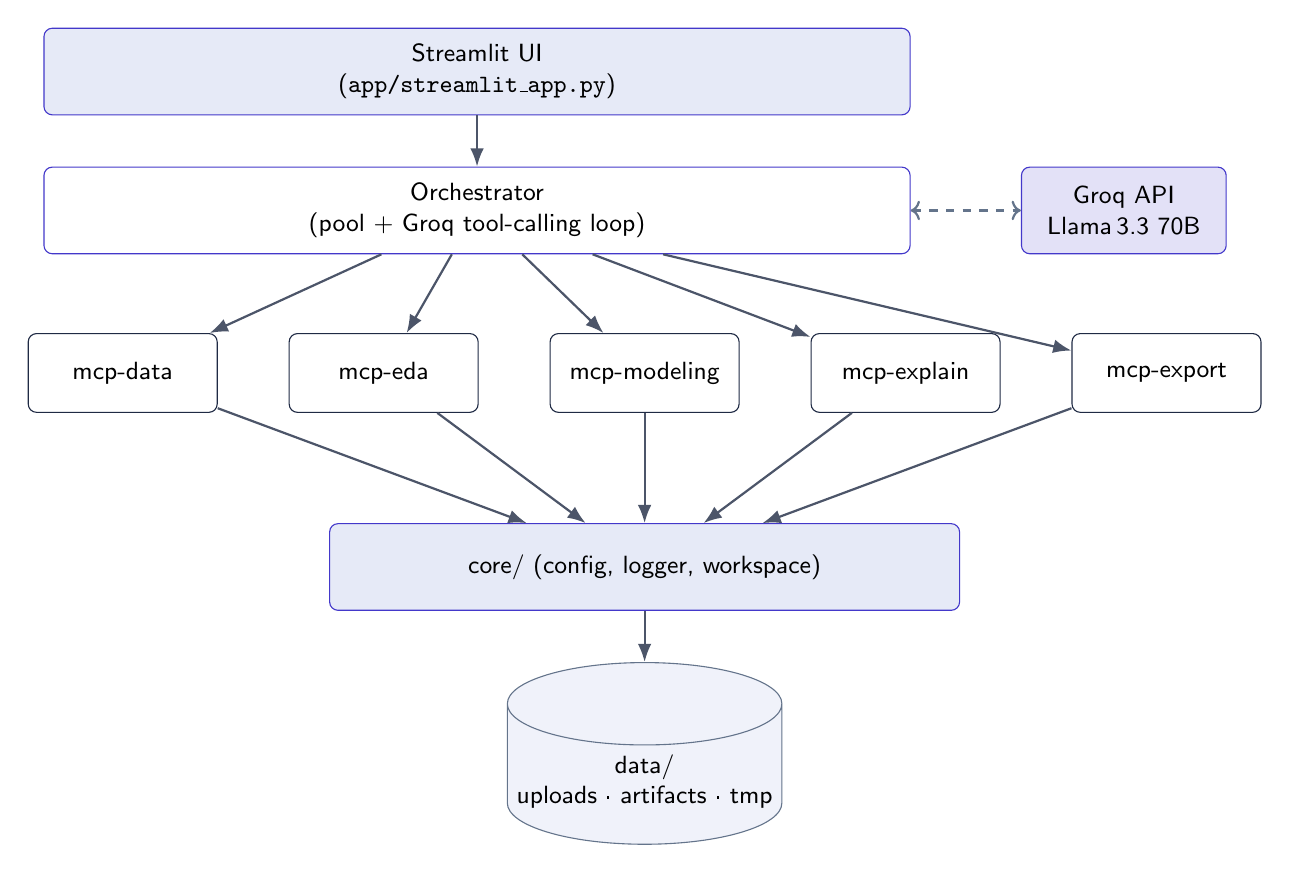
\begin{tikzpicture}[node distance=0.65cm and 0.9cm, font=\small\sffamily]

  \node[al-node, minimum width=11cm]                   (ui)   {Streamlit UI  \\ (\file{app/streamlit\_app.py})};

  \node[al-node, below=of ui, minimum width=11cm, fill=white]
                                                       (orch) {Orchestrator \\ (pool + Groq tool-calling loop)};

  \node[al-svc, below=1cm of orch, xshift=-4.5cm]      (s1)   {mcp-data};
  \node[al-svc, right=of s1]                           (s2)   {mcp-eda};
  \node[al-svc, right=of s2]                           (s3)   {mcp-modeling};
  \node[al-svc, right=of s3]                           (s4)   {mcp-explain};
  \node[al-svc, right=of s4]                           (s5)   {mcp-export};

  \node[al-node, below=1.4cm of s3, minimum width=8cm, fill=alSoft]
                                                       (core) {core/ (config, logger, workspace)};

  \node[al-store, below=of core]                       (fs)   {data/ \\ uploads · artifacts · tmp};

  \node[al-node, right=1.4cm of orch, fill=alAccent!15]
                                                       (llm)  {Groq API \\ Llama\,3.3 70B};

  \draw[al-flow] (ui)   -- (orch);
  \draw[al-flow] (orch) -- (s1);
  \draw[al-flow] (orch) -- (s2);
  \draw[al-flow] (orch) -- (s3);
  \draw[al-flow] (orch) -- (s4);
  \draw[al-flow] (orch) -- (s5);
  \draw[al-flow] (s1) -- (core);
  \draw[al-flow] (s2) -- (core);
  \draw[al-flow] (s3) -- (core);
  \draw[al-flow] (s4) -- (core);
  \draw[al-flow] (s5) -- (core);
  \draw[al-flow] (core) -- (fs);
  \draw[al-flow-dashed, <->] (orch.east) -- (llm.west);

\end{tikzpicture}
\caption{High-level architecture of \projname. Solid arrows carry
data or control in-process; the dashed arrow to the Groq API is the
only network dependency.}
\label{fig:high-level}
\end{figure}

\section{Runtime Model}
\label{sec:runtime}

The Streamlit script is the process entry point. It creates a
long-lived asyncio event loop in a daemon thread and constructs a
single \code{MCPClientPool}. The pool then registers the five
FastMCP servers and connects to each via \code{FastMCPTransport}.
Because the transport is in-process, no ports are opened and no
sockets are created --- the client's \code{call\_tool} coroutine
dispatches directly to the server's Python function via FastMCP's
internal message routing.

The Groq API is reached through the official \code{groq} Python
client, which internally uses \code{httpx}. The client is
instantiated per user turn (there is no persistent chat completion
stream). Each chat turn creates a fresh chat completions request in
streaming mode; the orchestrator consumes tokens and tool-call
deltas incrementally and dispatches tool invocations on the shared
event loop.

\section{Component Responsibilities}
\label{sec:responsibilities}

Table~\ref{tab:responsibilities} maps each component to its
responsibilities.

\begin{table}[H]
\centering
\caption{Components and responsibilities.}
\label{tab:responsibilities}
\small
\begin{tabularx}{\linewidth}{@{}lX@{}}
\toprule
\textbf{Component} & \textbf{Responsibilities} \\
\midrule
\file{core/config.py} & Loads settings from \code{.env}; exposes typed
attributes (\code{GROQ\_API\_KEY}, \code{GROQ\_MODEL},
\code{DATA\_DIR}, \code{MAX\_TOOL\_ITERATIONS}, \code{MAX\_UPLOAD\_MB});
computes derived paths. \\
\file{core/logger.py} & Named-logger factory writing to stderr. \\
\file{core/workspace.py} & Dataset save/list/resolve; artefact save;
artefact registry serialisation to \file{data/artifacts/\_index.json}. \\
\file{mcp\_servers/data.py} & Ingestion, preview, pandera-based schema
validation. \\
\file{mcp\_servers/eda.py} & Full EDA tool, standalone correlation
matrix tool, EDA prompt. \\
\file{mcp\_servers/modeling.py} & Parallel bake-off, Optuna sweep. \\
\file{mcp\_servers/explain.py} & SHAP calculation, native feature
importances. \\
\file{mcp\_servers/export.py} & Jupyter notebook generation, PDF
report generation. \\
\file{orchestrator/pool.py} & Client pool, service state, unified tool
schema, in-process routing, observer/SSE stream. \\
\file{orchestrator/loop.py} & Groq streaming loop, tool argument
accumulation, progress bridging, event yielding. \\
\file{app/streamlit\_app.py} & Layout, upload widget, chat, artefact
preview, tool catalog viewer, background loop management. \\
\bottomrule
\end{tabularx}
\end{table}

\section{Data Flow}
\label{sec:data-flow}

Figure~\ref{fig:data-flow} traces the flow of user data through the
system.

\begin{figure}[H]
\centering
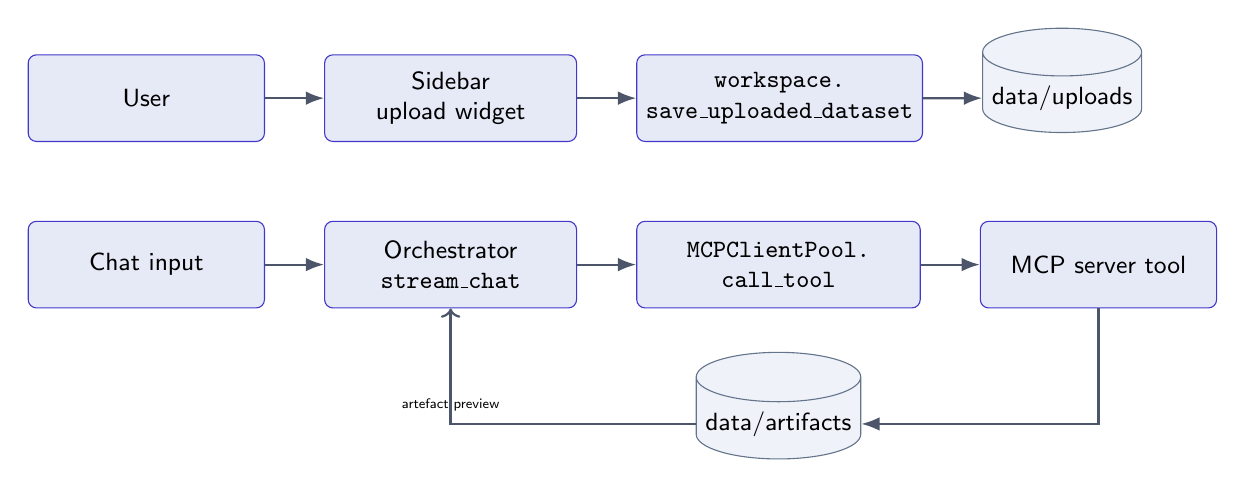
\begin{tikzpicture}[node distance=0.55cm and 0.75cm, font=\small\sffamily]
  \node[al-node, minimum width=3cm] (u) {User};
  \node[al-node, right=of u, minimum width=3.2cm] (up) {Sidebar \\ upload widget};
  \node[al-node, right=of up, minimum width=3.6cm] (ws) {\code{workspace.} \\ \code{save\_uploaded\_dataset}};
  \node[al-store, right=of ws] (fs) {data/uploads};

  \node[al-node, below=1cm of u, minimum width=3cm] (u2) {Chat input};
  \node[al-node, right=of u2, minimum width=3.2cm] (ol) {Orchestrator \\ \code{stream\_chat}};
  \node[al-node, right=of ol, minimum width=3.6cm] (mc) {\code{MCPClientPool.} \\ \code{call\_tool}};
  \node[al-node, right=of mc, minimum width=3cm] (srv) {MCP server tool};
  \node[al-store, below=of mc] (fs2) {data/artifacts};

  \draw[al-flow] (u)   -- (up);
  \draw[al-flow] (up)  -- (ws);
  \draw[al-flow] (ws)  -- (fs);
  \draw[al-flow] (u2)  -- (ol);
  \draw[al-flow] (ol)  -- (mc);
  \draw[al-flow] (mc)  -- (srv);
  \draw[al-flow] (srv.south) |- (fs2.east);
  \draw[al-flow, <-] (ol.south) |- (fs2.west) node[midway, above=1pt] {\tiny artefact preview};

\end{tikzpicture}
\caption{Data flow for uploads (top) and tool-invoked artefact
generation (bottom).}
\label{fig:data-flow}
\end{figure}

\section{Orchestration Flow}
\label{sec:orchestration-flow}

Figure~\ref{fig:orch-flow} sketches a single chat turn. The
orchestrator repeatedly calls the LLM, streams tokens back to the UI,
detects any \code{tool\_calls}, dispatches them through the pool,
appends the tool result to the message history, and re-invokes the
LLM until it produces a final message with no further tool calls or
the iteration limit is reached.

\begin{figure}[H]
\centering
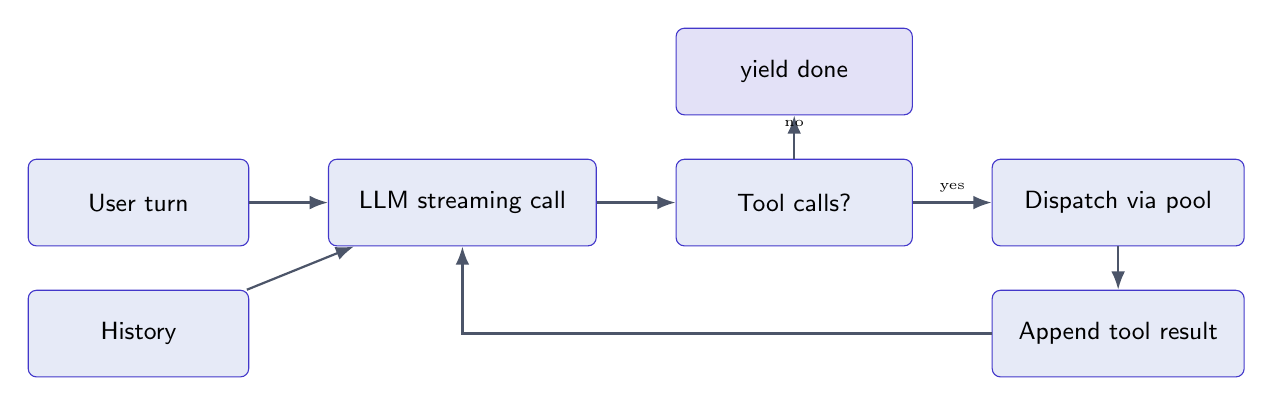
\begin{tikzpicture}[node distance=0.55cm and 1cm, font=\small\sffamily]
  \node[al-node, minimum width=2.8cm]                    (u)  {User turn};
  \node[al-node, below=of u, minimum width=2.8cm]        (h)  {History};
  \node[al-node, right=of u, minimum width=3.4cm]        (llm){LLM streaming call};
  \node[al-node, right=of llm, minimum width=3cm]        (dec){Tool calls?};
  \node[al-node, above=of dec, minimum width=3cm,
        fill=alAccent!15]                                 (done){yield done};
  \node[al-node, right=of dec, minimum width=3.2cm]      (dis){Dispatch via pool};
  \node[al-node, below=of dis, minimum width=3.2cm]      (rec){Append tool result};

  \draw[al-flow] (u)  -- (llm);
  \draw[al-flow] (h)  -- (llm);
  \draw[al-flow] (llm)-- (dec);
  \draw[al-flow] (dec)-- node[above,font=\tiny]{no} (done);
  \draw[al-flow] (dec)-- node[above,font=\tiny]{yes} (dis);
  \draw[al-flow] (dis)-- (rec);
  \draw[al-flow] (rec.west) -| (llm.south);
\end{tikzpicture}
\caption{Orchestration loop for a single user turn.}
\label{fig:orch-flow}
\end{figure}

\section{Artefact Flow}
\label{sec:artefact-flow}

Every generated file follows the same lifecycle:
\begin{enumerate}[leftmargin=1.4em]
  \item A tool writes the file into its private scratch directory
        under \file{data/tmp/<subdir>/}.
  \item The tool calls \code{save\_artifact(local\_path, kind,
        metadata)} in \file{core/workspace.py}.
  \item \code{save\_artifact} \emph{moves} the file to
        \file{data/artifacts/<category>/<uuid>\_\_<name>}, assigns a
        UUID, computes the MIME type, and appends a record to
        \file{data/artifacts/\_index.json}.
  \item The tool returns the resulting \code{artifact\_id} and
        \code{path} to the orchestrator, which surfaces them in the
        tool result.
  \item The Streamlit \emph{Artifacts} tab reads
        \code{list\_artifacts()} and renders each artefact according
        to its MIME type (image preview, dataframe preview for
        parquet, download button for PDFs).
\end{enumerate}

The kind-to-category mapping is a small dictionary in
\file{core/workspace.py}; adding a new artefact category requires only
adding one entry.

\section{Failure Modes and Graceful Degradation}
\label{sec:failures}

The pool tracks per-service state (\code{online}, \code{offline},
\code{processing}, \code{error}) and surfaces it in the sidebar. If
a specific tool raises an exception, the orchestrator captures the
exception message, returns it to the LLM as the tool result, and
allows the LLM to react (e.g.\ by picking a different tool or asking
the user to clarify). When the Groq API returns \code{429}, the
underlying \code{groq} client retries with exponential back-off. When
the API key is missing, the orchestrator emits an
\code{\{"type": "error"\}} event and the Streamlit UI renders it as
a red banner without crashing.

\chapter{Platform Design}
\label{ch:design}

Where Chapter~\ref{ch:arch} presented the architecture at the level
of boxes and arrows, this chapter describes each module in terms of
its Python types, key responsibilities, and design rationale. Every
reference in this chapter points to a real file in the repository.

\section{Project Structure}
\label{sec:project-structure}

\begin{lstlisting}[style=alBash, caption={Top-level project structure.},
                    label={lst:tree}]
automl-mcp-platform/
|-- app/
|   |-- streamlit_app.py     # Streamlit entrypoint (thin UI)
|   `-- components/          # reserved for render helpers
|-- core/
|   |-- config.py            # pydantic-settings + derived paths
|   |-- logger.py            # named-logger factory
|   `-- workspace.py         # datasets + artifacts registry (local FS)
|-- mcp_servers/
|   |-- data.py              # ingest, list, pandera validation
|   |-- eda.py               # run_full_eda, correlation, prompt
|   |-- modeling.py          # bake-off + Optuna sweep
|   |-- explain.py           # SHAP + native feature importances
|   `-- export.py            # Jupyter notebook + PDF report
|-- orchestrator/
|   |-- pool.py              # MCPClientPool over FastMCPTransport
|   `-- loop.py              # Groq tool-calling loop
|-- data/{uploads,artifacts,tmp}/
|-- requirements.txt
|-- .env.example
`-- README.md
\end{lstlisting}

The choice to keep four sibling top-level packages
(\code{app}, \code{core}, \code{mcp\_servers}, \code{orchestrator})
rather than nesting them under a single \code{src/} package is
deliberate: it makes the dependency graph flat and readable
(\code{app $\rightarrow$ orchestrator $\rightarrow$ mcp\_servers $\rightarrow$ core}),
and it keeps the Streamlit entrypoint invokable with
\code{streamlit run app/streamlit\_app.py} without any wrapper.

\section{Configuration}
\label{sec:config}

Configuration is centralised in \file{core/config.py}:

\begin{lstlisting}[caption={\file{core/config.py} (extract).},
                    label={lst:config}]
class Settings(BaseSettings):
    GROQ_API_KEY: str = ""
    GROQ_MODEL: str = "llama-3.3-70b-versatile"
    MAX_TOOL_ITERATIONS: int = 8
    MAX_UPLOAD_MB: int = 200
    DATA_DIR: str = str(REPO_ROOT / "data")

    @property
    def data_path(self) -> Path: ...
    @property
    def uploads_path(self) -> Path: ...
    @property
    def artifacts_path(self) -> Path: ...
    @property
    def tmp_path(self) -> Path: ...
\end{lstlisting}

Every setting is env-driven through \code{pydantic-settings}
\citep{pydantic}. Derived paths are exposed as properties that
create the directory on first access, so no module has to worry
about directory existence. Appendix~\ref{app:config} lists every
setting with its default and description.

\section{Logging}
\label{sec:logging}

\file{core/logger.py} exposes a single \code{get\_logger(name)}
factory that returns a name-scoped logger with a compact stderr
formatter. This keeps log output consistent across every module and
avoids the common ``duplicate handler'' problem when Streamlit
re-runs the script:

\begin{lstlisting}[caption={\file{core/logger.py}.},label={lst:logger}]
def get_logger(name: str) -> logging.Logger:
    logger = logging.getLogger(name)
    if logger.handlers:
        return logger  # idempotent
    logger.setLevel(logging.INFO)
    handler = logging.StreamHandler(sys.stderr)
    handler.setFormatter(logging.Formatter(
        fmt="%(asctime)s | %(levelname)-7s | %(name)s | %(message)s",
        datefmt="%H:%M:%S"))
    logger.addHandler(handler)
    logger.propagate = False
    return logger
\end{lstlisting}

\section{The Workspace Module}
\label{sec:workspace}

\file{core/workspace.py} is the sole persistence layer. It contains
two dataclasses --- \code{DatasetRecord} and \code{ArtifactRecord}
--- and a small set of pure functions.

\paragraph{Dataset operations.}
\code{save\_uploaded\_dataset(filename, data, \dots)} writes raw
bytes into \file{data/uploads/}, deduplicating filenames by appending
a Unix timestamp when necessary, and returns a \code{DatasetRecord}
with a UUID and populated row/column metadata (if supplied by the
caller). \code{list\_datasets()} enumerates the uploads directory and
returns dictionaries sorted by modification time.
\code{resolve\_dataset(file\_ref)} accepts either an absolute path or
a base filename and returns the resolved \code{Path}, raising
\code{FileNotFoundError} with a helpful message when the file is not
present.

\paragraph{Artefact operations.}
\code{save\_artifact(local\_path, kind, metadata=\dots, move=True)}
is the single entry point that every MCP tool uses. It:
\begin{enumerate}[leftmargin=1.4em]
  \item Resolves the target category from a kind-to-category
        dictionary (\code{plot} $\rightarrow$ \code{plots},
        \code{model} $\rightarrow$ \code{models}, etc.).
  \item Assigns a UUID and constructs a destination path of the form
        \code{data/artifacts/<category>/<uuid[:8]>\_\_<safe\_name>}.
  \item Moves or copies the file, computes MIME type via
        \code{mimetypes}, and appends a JSON record to
        \file{data/artifacts/\_index.json}.
\end{enumerate}
The registry is a plain JSON array to keep the code trivial;
switching to SQLite or an experiment tracker (Section~\ref{sec:future-mlops})
requires changing only this file.

\section{The MCP Servers}
\label{sec:servers-design}

Each server module follows the same template:

\begin{lstlisting}[caption={MCP server module template.},
                    label={lst:server-template}]
mcp = FastMCP(name="mcp-<service>")

@mcp.tool
def <tool_name>(arg1: <T1>, arg2: <T2> = <default>, ...) -> dict[str, Any]:
    """Short description used as the LLM-visible tool description.

    Args:
        arg1: ...
        arg2: ...
    """
    ...
    return {"...": ...}
\end{lstlisting}

Tools whose work is compute-bound or IO-bound are declared
\code{async def} and additionally receive a \code{ctx: Context}
parameter through which they emit progress with
\code{ctx.report\_progress(current, total, message)}.

\subsection{\svc{mcp-data}}
Three tools: \tool{list\_uploaded\_files},
\tool{ingest\_dataset}, \tool{validate\_schema\_with\_pandera}.
The validation tool infers a \code{pandera.DataFrameSchema} by
walking each column: numeric columns receive an \code{in\_range} check,
low-cardinality string columns receive an \code{isin} check, and
nullability follows from observed NaN values. The tool returns the
first 50 failure cases (column, check, offending value, index) to
make debugging tractable.

\subsection{\svc{mcp-eda}}
Two tools: \tool{run\_full\_eda} and \tool{render\_correlation\_matrix},
and one prompt: \tool{eda\_deep\_dive}. The full EDA tool renders
three PNGs into a per-service scratch directory
(\file{data/tmp/eda/}) before handing them to
\code{save\_artifact}. Correlation entries above $|\rho|\ge 0.6$ are
returned as ``strong correlations'' so that the LLM can surface them
in prose.

\subsection{\svc{mcp-modeling}}
Two tools: \tool{run\_parallel\_bake\_off} and
\tool{trigger\_hyperparameter\_sweep}.
The bake-off constructs a shared
\code{ColumnTransformer} preprocessor and spawns a
\code{ThreadPoolExecutor} with up to four workers, one per
candidate. Each worker runs $k$-fold cross-validation with either
\code{f1\_weighted} or \code{r2}, then refits on the full training
split and evaluates on the held-out test split. Champion selection
uses the primary metric (F1 for classification, $R^2$ for
regression). The champion pipeline is serialised with \code{joblib}
along with the feature columns, problem type, and target column, and
persisted as a \code{model} artefact. A 500-row sample of
\code{X\_train} is written as parquet and persisted as an
\code{xtrain\_sample} artefact for downstream SHAP.

\subsection{\svc{mcp-explain}}
Two tools: \tool{calculate\_shap\_values} and
\tool{generate\_feature\_importance\_plot}.
Both tools read the champion artefact by ID via
\code{workspace.artifact\_path}, so the ID plumbed from the bake-off
result is the only coupling between the modelling and explainability
stages.

\subsection{\svc{mcp-export}}
Two tools: \tool{generate\_jupyter\_notebook} and
\tool{compile\_pdf\_report}. Notebooks are built as pure Python
dictionaries following the nbformat schema and serialised to disk
with \code{json.dumps}. PDFs are built with ReportLab
\citep{reportlab}: a title block, a summary paragraph, a leaderboard
table, and an optional notes section.

\section{Orchestration Design}
\label{sec:orch-design}

Two responsibilities live in \file{orchestrator/}: aggregating the
tools into a single catalog (\file{pool.py}) and iterating on the
LLM's tool-call loop (\file{loop.py}).

\subsection{The Pool}
\label{sec:pool-design}

\code{MCPClientPool} maintains three registries: \code{tool\_index}
(tool name $\to$ owning service name), \code{tool\_schemas}
(OpenAI-compatible schema list ready to be passed to Groq), and
\code{prompt\_index}. Registries are rebuilt on start-up and can be
refreshed after a service reconnect.

A key design decision is name-collision handling. If two servers
register a tool with the same name, the second one is registered
under a canonical name of the form
\code{<service>\_\_<original\_name>}. This is deliberately loud so
that the developer notices and renames.

\subsection{The Loop}
\label{sec:loop-design}

\code{stream\_chat} is an asynchronous generator of event dicts.
Each iteration of the outer \code{for} loop is one Groq streaming
call. The loop accumulates \code{tool\_calls} chunks, materialises
them into a list, executes them (with per-tool progress bridged
through an \code{asyncio.Queue}), appends the tool results back to
the message history, and re-invokes the LLM. The loop terminates
either when Groq emits no \code{tool\_calls} in an iteration or when
\code{MAX\_TOOL\_ITERATIONS} is reached.

The generator emits six event kinds --- \code{token},
\code{tool\_start}, \code{tool\_progress}, \code{tool\_end},
\code{done}, \code{error} --- documented in
Section~\ref{sec:event-schema}. This design is intentionally
UI-agnostic: any consumer (CLI, Jupyter widget, Streamlit,
FastAPI-over-SSE) can subscribe.

\section{Streamlit Front-end}
\label{sec:st-design}

The UI has three tabs: \emph{Chat}, \emph{Artifacts}, and
\emph{Tools}. A sidebar contains the upload widget, the active
dataset selector, and a live service-status list built from
\code{pool.snapshot()}.

To bridge Streamlit's synchronous execution model with the async
orchestrator, the UI creates a single \code{PoolRunner} object cached
via \code{st.cache\_resource}. \code{PoolRunner} owns a dedicated
event loop running in a daemon thread and exposes a
\code{stream\_events(query, active\_file, history)} method that
returns a \code{queue.Queue}. Each user turn consumes the queue in
the main thread and updates Streamlit placeholders in place. This
gives the appearance of real-time streaming without pushing async
into the Streamlit script.

\section{Extensibility}
\label{sec:extensibility}

Adding a new capability follows a strict recipe:

\begin{enumerate}[leftmargin=1.4em]
  \item Add a \code{@mcp.tool}-decorated function to the appropriate
        \file{mcp\_servers/<service>.py} (or create a new server
        module and register it in
        \file{orchestrator/pool.py::register\_default\_servers}).
  \item If the tool generates a new kind of file, add a
        kind-to-category entry to \code{\_KIND\_TO\_CATEGORY} in
        \file{core/workspace.py}.
  \item Optionally, add a friendly label to \code{TOOL\_LABELS} in
        \file{orchestrator/loop.py}.
\end{enumerate}

No change is required to the Streamlit UI or to the orchestration
loop.

\chapter{MCP and Agent Architecture}
\label{ch:mcp}

This chapter dives into the specific integration between the Model
Context Protocol (MCP) and the Groq-hosted LLM agent that drives the
platform. The material is organised bottom-up: protocol primitives,
tool discovery, tool invocation, agent decision flow, and
extensibility.

\section{MCP in One Page}
\label{sec:mcp-onepager}

MCP \citep{mcpSpec2024, anthropic2024mcp} is a JSON-RPC 2.0 protocol
in which an \emph{MCP host} (typically an LLM application) connects
to one or more \emph{MCP servers}, each of which exposes some
combination of tools, resources, and prompts. Communication happens
through a \emph{transport}. The reference implementation uses stdio
or WebSockets, but FastMCP \citep{fastmcp} also provides
\code{FastMCPTransport}, which runs the entire client/server exchange
as ordinary \code{async} method calls inside the same Python
process. \projname{} uses \code{FastMCPTransport} exclusively.

\section{The In-Process Pool}
\label{sec:in-process-pool}

Figure~\ref{fig:pool} shows the \code{MCPClientPool} at startup. The
pool wraps each FastMCP server in a \code{Client(FastMCPTransport(server))},
enters the client's async context in an \code{AsyncExitStack}, and
records the state.

\begin{figure}[H]
\centering
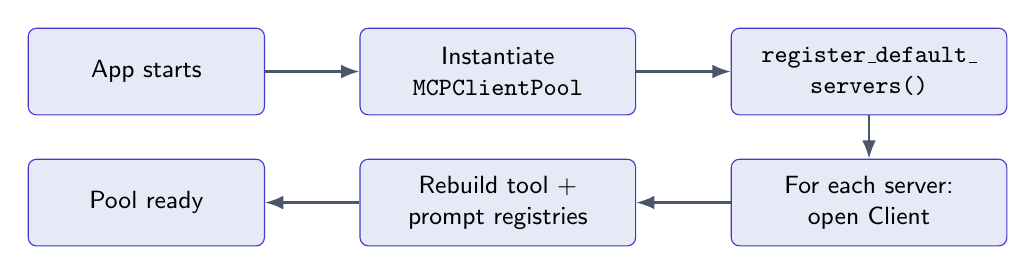
\begin{tikzpicture}[node distance=0.55cm and 1.2cm, font=\small\sffamily]
  \node[al-node, minimum width=3cm]                     (a) {App starts};
  \node[al-node, right=of a, minimum width=3.5cm]       (b) {Instantiate \\ \code{MCPClientPool}};
  \node[al-node, right=of b, minimum width=3.5cm]       (c) {\code{register\_default\_} \\ \code{servers()}};
  \node[al-node, below=of c, minimum width=3.5cm]       (d) {For each server: \\ open Client};
  \node[al-node, left=of d, minimum width=3.5cm]        (e) {Rebuild tool + \\ prompt registries};
  \node[al-node, left=of e, minimum width=3cm]          (f) {Pool ready};

  \draw[al-flow] (a) -- (b);
  \draw[al-flow] (b) -- (c);
  \draw[al-flow] (c) -- (d);
  \draw[al-flow] (d) -- (e);
  \draw[al-flow] (e) -- (f);
\end{tikzpicture}
\caption{Pool startup sequence.}
\label{fig:pool}
\end{figure}

Once startup finishes, the pool exposes four public interfaces:

\begin{itemize}[leftmargin=1.4em]
  \item \code{tool\_schemas} --- a list of OpenAI-compatible function
        schemas ready to hand to the LLM.
  \item \code{call\_tool(name, arguments, progress\_handler)} ---
        routes to the correct client and forwards progress events.
  \item \code{get\_prompt(name, arguments)} --- retrieves a
        parameterised prompt template.
  \item \code{snapshot()} --- an inspectable dictionary of service
        state, tool counts, and prompt metadata (used by the sidebar
        health panel).
\end{itemize}

\section{Tool Discovery}
\label{sec:discovery}

Immediately after all clients connect, \code{\_rebuild\_registries}
loops through the clients and calls \code{list\_tools},
\code{list\_resources} (best-effort), and \code{list\_prompts}
(best-effort). For each tool it constructs an OpenAI-compatible
schema of the form
\begin{lstlisting}[caption={Schema shape passed to the Groq API.},
                    label={lst:openai-schema}]
{
  "type": "function",
  "function": {
    "name":        "<tool_name>",
    "description": "<tool.description>",
    "parameters":  <tool.inputSchema>       # JSON Schema
  }
}
\end{lstlisting}
The pool preserves the natural-language tool description generated by
FastMCP from the Python docstring; this is what the LLM sees when it
decides whether a tool is relevant.

\section{Tool Invocation Sequence}
\label{sec:invocation}

Figure~\ref{fig:seq} shows a single tool call from the LLM's
perspective. The sequence is compressed --- in a real turn each of
the arrows is streamed piecewise.

\begin{figure}[H]
\centering
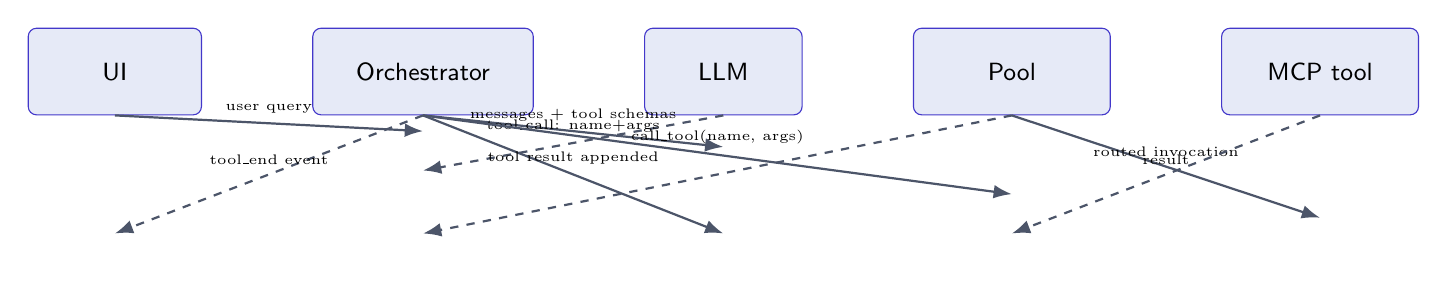
\begin{tikzpicture}[node distance=0.4cm and 1.4cm, font=\small\sffamily]
  \node[al-node, minimum width=2.2cm] (ui) {UI};
  \node[al-node, right=of ui, minimum width=2.8cm] (or) {Orchestrator};
  \node[al-node, right=of or, minimum width=2cm] (llm) {LLM};
  \node[al-node, right=of llm, minimum width=2.5cm] (po) {Pool};
  \node[al-node, right=of po, minimum width=2.5cm] (srv) {MCP tool};

  \node[below=1.6cm of ui, minimum width=0.1cm] (ui2){};
  \node[below=1.6cm of or, minimum width=0.1cm] (or2){};
  \node[below=1.6cm of llm, minimum width=0.1cm] (llm2){};
  \node[below=1.6cm of po, minimum width=0.1cm] (po2){};
  \node[below=1.6cm of srv, minimum width=0.1cm] (srv2){};

  \draw[al-flow] (ui.south)  -- ($(or.south)+(0,-0.2)$) node[midway,above,font=\tiny]{user query};
  \draw[al-flow] (or.south)  -- ($(llm.south)+(0,-0.4)$) node[midway,above,font=\tiny]{messages + tool schemas};
  \draw[al-flow, dashed] (llm.south) -- ($(or.south)+(0,-0.7)$) node[midway,above,font=\tiny]{tool\_call: name+args};
  \draw[al-flow] (or.south)  -- ($(po.south)+(0,-1.0)$) node[midway,above,font=\tiny]{call\_tool(name, args)};
  \draw[al-flow] (po.south)  -- ($(srv.south)+(0,-1.3)$) node[midway,above,font=\tiny]{routed invocation};
  \draw[al-flow, dashed] (srv.south) -- ($(po.south)+(0,-1.5)$) node[midway,above,font=\tiny]{result};
  \draw[al-flow, dashed] (po.south) -- ($(or.south)+(0,-1.5)$);
  \draw[al-flow] (or.south)  -- ($(llm.south)+(0,-1.5)$) node[midway,above,font=\tiny]{tool result appended};
  \draw[al-flow, dashed] (or.south) -- ($(ui.south)+(0,-1.5)$) node[midway,above,font=\tiny]{tool\_end event};

\end{tikzpicture}
\caption{Single tool-call round trip. Dashed arrows indicate
streamed responses.}
\label{fig:seq}
\end{figure}

\section{Progress Bridging}
\label{sec:progress}

MCP tools can report progress by calling
\code{ctx.report\_progress(current, total, message)}. FastMCP
delivers these to a progress handler supplied by the client. The
orchestrator installs a handler that pushes each event into an
\code{asyncio.Queue}. During tool execution, the orchestrator polls
the queue with a short timeout and yields any accumulated events as
\code{tool\_progress} events. This is what enables the ``training
model 3/4 --- 42\% complete'' line that the Streamlit UI renders in
place.

\section{The Agent Decision Flow}
\label{sec:agent-flow}

The agent is a single-turn planner in the ReAct style
\citep{yao2023react}: it receives (i)~a system prompt that describes
its role and the tool catalog, (ii)~the conversation history, and
(iii)~the current user query, and it emits either plain text or a
tool call. The system prompt (constructed by
\code{orchestrator/loop.py::\_build\_messages}) instructs the model
to:

\begin{itemize}[leftmargin=1.4em]
  \item Prefer the \emph{active dataset} named in context when the
        user says ``my data'' or ``the dataset''.
  \item Never invent numerical claims --- always ground them in tool
        results.
  \item After a bake-off succeeds, proactively compute SHAP values
        with the returned \code{model\_id} and
        \code{x\_train\_sample\_id}.
  \item Prefer short paragraphs and light bullets.
\end{itemize}

Multi-step behaviour is achieved by allowing the LLM to emit
\emph{multiple} tool calls per turn and by permitting up to
\code{MAX\_TOOL\_ITERATIONS} loops, so a request such as ``run EDA
and then train a model'' typically fires 3--5 tools in a single
user turn.

\section{Security Considerations}
\label{sec:security-mcp}

Because \projname{} is a single-user local tool, the threat model is
lightweight, but a few observations are worth recording.

\begin{itemize}[leftmargin=1.4em]
  \item \textbf{Prompt injection.} The tool descriptions are trusted
        (they are versioned code), but the \emph{results} of tools
        are attacker-influenced (they may contain data from an
        uploaded CSV). The system does not currently sanitise
        tool results before feeding them back to the LLM; a
        malicious CSV cell could in principle contain instructions
        aimed at the model. In practice this is mitigated by
        showing the entire tool result to the user in an expander;
        no unattended automation occurs.
  \item \textbf{Filesystem writes.} Every write goes through
        \code{workspace.save\_artifact}, which sanitises the filename
        via \code{\_safe\_stem} (only alphanumerics, dashes,
        underscores, and dots survive). This prevents path traversal
        in \code{data/artifacts/}.
  \item \textbf{Arbitrary code execution.} The platform never
        \code{exec}s LLM-produced code. The LLM can only invoke
        pre-defined tools with typed arguments.
  \item \textbf{Network.} The only outbound network call is to Groq;
        no inbound network is opened.
\end{itemize}

\section{Extensibility}
\label{sec:mcp-extensibility}

The MCP layer is trivially extensible:

\begin{enumerate}[leftmargin=1.4em]
  \item Add a new tool by decorating a function with
        \code{@mcp.tool} in one of the existing servers.
  \item Add a new server by creating a new
        \file{mcp\_servers/<name>.py} module and registering its
        \code{mcp} instance in
        \code{register\_default\_servers()}.
  \item Add a prompt template by decorating a function with
        \code{@mcp.prompt}; it becomes visible under
        \code{pool.prompts\_meta}.
\end{enumerate}

No changes to \file{orchestrator/loop.py} or
\file{app/streamlit\_app.py} are required. The new tool will appear
in the LLM's tool schema list on the next start-up.

\section{Comparison to HTTP-Based MCP}
\label{sec:vs-http}

MCP is more commonly deployed over stdio or Streamable HTTP. The
in-process transport has three practical advantages for a research
platform:

\begin{itemize}[leftmargin=1.4em]
  \item No port management, no shutdown races, no partial startup.
  \item Zero-copy Python object passing between client and server.
  \item Perfect traceability in a Python debugger --- each tool
        invocation is a normal call stack.
\end{itemize}

The disadvantages (no cross-language servers, no independent scaling
per service) are acceptable for a single-user tool. Because the
protocol contract is unchanged, the servers can be re-hosted over
HTTP simply by swapping the transport in \code{register\_default\_servers}.

\chapter{The AutoML Pipeline}
\label{ch:pipeline}

Chapter~\ref{ch:arch} explained \emph{how} components communicate;
this chapter explains \emph{what} the platform actually does with a
dataset. The pipeline is written as if the LLM issues each tool call
manually, because in practice the LLM composes them in exactly this
order.

\section{Pipeline Overview}
\label{sec:pipeline-overview}

\begin{figure}[H]
\centering
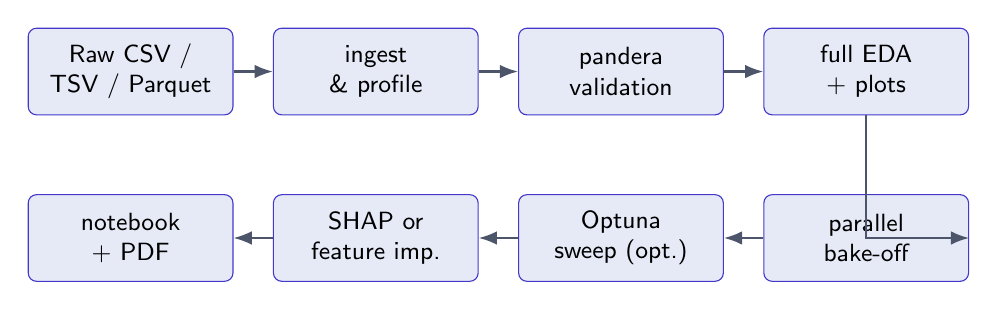
\begin{tikzpicture}[node distance=0.5cm and 0.5cm, font=\small\sffamily]
  \node[al-node, minimum width=2.6cm]                              (raw){Raw CSV / \\ TSV / Parquet};
  \node[al-node, right=of raw, minimum width=2.6cm]                (ing){ingest \\ \& profile};
  \node[al-node, right=of ing, minimum width=2.6cm]                (val){pandera \\ validation};
  \node[al-node, right=of val, minimum width=2.6cm]                (eda){full EDA \\ + plots};
  \node[al-node, below=1cm of eda, minimum width=2.6cm]            (bak){parallel \\ bake-off};
  \node[al-node, left=of bak, minimum width=2.6cm]                 (hpo){Optuna \\ sweep (opt.)};
  \node[al-node, left=of hpo, minimum width=2.6cm]                 (shap){SHAP or \\ feature imp.};
  \node[al-node, left=of shap, minimum width=2.6cm]                (exp){notebook \\ + PDF};

  \draw[al-flow] (raw)--(ing);
  \draw[al-flow] (ing)--(val);
  \draw[al-flow] (val)--(eda);
  \draw[al-flow] (eda.south) |- (bak.east);
  \draw[al-flow] (bak)--(hpo);
  \draw[al-flow] (hpo)--(shap);
  \draw[al-flow] (shap)--(exp);
\end{tikzpicture}
\caption{End-to-end tabular AutoML pipeline realised by \projname.}
\label{fig:pipeline}
\end{figure}

Each box maps to one or two MCP tools; the arrows are optional to the
extent that the LLM may skip stages (e.g.\ if the user only asks for
EDA). \impl{} labels apply to every stage --- there is no ``proposed
but unimplemented'' step in Figure~\ref{fig:pipeline}.

\section{Stage 1: Ingestion}
\label{sec:stage-ingest}

The user uploads a file via the Streamlit sidebar; bytes are handed
to \code{workspace.save\_uploaded\_dataset}, which writes to
\file{data/uploads/<safe\_name>}.

The LLM then invokes \tool{ingest\_dataset(file\_path)}. The tool
delegates to \code{workspace.resolve\_dataset} to obtain the local
path, reads the file with \code{pandas.read\_csv}
(or \code{read\_parquet} / \code{read\_json}), and returns:

\begin{itemize}[leftmargin=1.4em]
  \item File name, format, and shape.
  \item Memory footprint in KB.
  \item Column names and dtypes.
  \item Head preview (default 5 rows).
  \item Total missing count and duplicate-row count.
\end{itemize}

This response is small enough to fit comfortably in the LLM context
and gives the model everything it needs to reason about subsequent
questions --- ``does the target column exist?'', ``is this
classification or regression?'', ``what fraction is missing?''.

\section{Stage 2: Schema Validation}
\label{sec:stage-validate}

\tool{validate\_schema\_with\_pandera(file\_path, expected\_columns,
strict\_dtypes)} infers a pandera schema and validates the frame
against it in lazy mode. Rules are constructed per column as follows:

\begin{itemize}[leftmargin=1.4em]
  \item Numeric columns receive
        \code{pa.Check.in\_range(min, max)}.
  \item Low-cardinality string columns ($\le 20$ uniques) receive
        \code{pa.Check.isin(allowed\_categories)}.
  \item Nullability follows from observed missing values.
\end{itemize}

The tool returns the inferred rules, whether validation succeeded,
and up to 50 failure cases. This is used by the LLM to warn the user
about outliers, unexpected string values, or off-range numeric
readings before any modelling is done.

\section{Stage 3: Exploratory Data Analysis}
\label{sec:stage-eda}

\tool{run\_full\_eda(file\_path, target\_column)} produces:

\begin{enumerate}[leftmargin=1.4em]
  \item Descriptive statistics per numeric column: mean, std, min,
        Q25, median, Q75, max, IQR, skewness, IQR-outlier count.
  \item Descriptive statistics per categorical column: unique count,
        top value, top frequency, top-5 values.
  \item Missing-value summary per column and overall.
  \item Three matplotlib plots saved as PNG artefacts:
        \begin{itemize}[leftmargin=1.2em]
          \item Correlation matrix (\emph{if} $\ge 2$ numeric cols).
          \item Small multiple of histograms for the first
                12 numeric columns.
          \item Bar chart of missing percentages (\emph{if} any
                missing values exist).
        \end{itemize}
  \item Optional target analysis if the user supplied a
        \code{target\_column}.
\end{enumerate}

\tool{render\_correlation\_matrix} produces a standalone correlation
heatmap with Pearson, Spearman, or Kendall as requested, and reports
the top pairs with $|\rho| \ge 0.6$.

\section{Stage 4: Model Selection --- The Bake-Off}
\label{sec:stage-bakeoff}

The bake-off is the analytical heart of the platform.
\tool{run\_parallel\_bake\_off(file\_path, target\_column, test\_size,
cv, random\_state)} performs the following procedure.

\begin{algorithm}[H]
\caption{Parallel bake-off (\code{mcp\_servers/modeling.py}).}
\label{alg:bakeoff}
\begin{algorithmic}[1]
\Require dataset $\mathcal{D}$, target $t$, test size $s$, folds $k$, seed $\sigma$
\State drop rows with NaN in $t$; abort if $t \notin \mathcal{D}$
\State $y \gets \mathcal{D}[t]$; if $y$ non-numeric $\Rightarrow$ label-encode
\State detect problem type from $y$ (classification if $|\text{unique}| \le \max(20, 0.05n)$ or non-numeric; else regression)
\State build \code{ColumnTransformer}: median-impute+scale numerics, most-frequent+one-hot categoricals
\State stratified split $(X_{tr}, X_{te}, y_{tr}, y_{te})$
\State $\mathcal{M} \gets \{\text{RandomForest}, \text{XGBoost}, \text{LightGBM}, \text{baseline}\}$ (LR or Ridge)
\ForAll{$m \in \mathcal{M}$ in parallel (thread pool, max 4)}
  \State $\text{cv}_m \gets \operatorname{cross\_val\_score}(\text{Pipe}(pre, m), X_{tr}, y_{tr}, cv=k, \text{scoring}=\text{primary})$
  \State refit on $(X_{tr}, y_{tr})$; predict on $X_{te}$
  \State compute accuracy \& $F_1$ (classification) or RMSE \& $R^2$ (regression); record train time
\EndFor
\State sort leaderboard by primary metric descending; abort if all failed
\State $\text{champion} \gets \arg\max$
\State persist champion pipeline (joblib) and $X_{tr}[0{:}500]$ sample (parquet) as artefacts
\State \Return leaderboard, champion, model\_id, x\_train\_sample\_id
\end{algorithmic}
\end{algorithm}

The primary metric is F1-weighted for classification and $R^2$ for
regression. The choice of a small candidate set (four models) is
deliberate: it favours interpretability and short training times
over exhaustive search, which is appropriate for the ``upload a CSV
and get a baseline'' use case.

\section{Stage 5: Hyperparameter Optimisation (Optional)}
\label{sec:stage-hpo}

\tool{trigger\_hyperparameter\_sweep(file\_path, target\_column,
model\_family, time\_budget\_seconds, cv, random\_state)} performs a
TPE-based Optuna study on one of RandomForest, XGBoost, or LightGBM.
The search space is defined inside the objective function
(``define-by-run''):

\begin{itemize}[leftmargin=1.4em]
  \item \textbf{RandomForest:} \code{n\_estimators} $\in [100, 600]$,
        \code{max\_depth} $\in [3, 30]$, \code{min\_samples\_split}
        $\in [2, 20]$.
  \item \textbf{XGBoost:} \code{n\_estimators} $\in [100, 600]$,
        \code{max\_depth} $\in [3, 12]$, \code{learning\_rate}
        $\in [10^{-2}, 3\!\cdot\!10^{-1}]$ (log-uniform),
        \code{subsample} and \code{colsample\_bytree} $\in [0.6, 1.0]$.
  \item \textbf{LightGBM:} \code{n\_estimators} $\in [100, 600]$,
        \code{num\_leaves} $\in [15, 127]$, \code{learning\_rate}
        $\in [10^{-2}, 3\!\cdot\!10^{-1}]$ (log-uniform),
        \code{feature\_fraction} $\in [0.6, 1.0]$.
\end{itemize}

The study is bounded by wall-clock time; progress is streamed at
2-second intervals with the best value observed so far.

\section{Stage 6: Explainability}
\label{sec:stage-explain}

The champion model is loaded by ID via
\code{workspace.artifact\_path}. \tool{calculate\_shap\_values}
picks an explainer based on the class name of the underlying
estimator:

\begin{itemize}[leftmargin=1.4em]
  \item Tree-family (\code{Forest}, \code{XGB}, \code{LGBM},
        \code{GradientBoosting}) $\rightarrow$ \code{TreeExplainer}
        \citep{lundberg2020treeshap}.
  \item Otherwise $\rightarrow$ \code{KernelExplainer} against a
        100-sample background.
\end{itemize}

The tool renders \code{shap.summary\_plot} and stores it as a plot
artefact, and returns a top-20 mean-absolute-SHAP ranking.

\tool{generate\_feature\_importance\_plot} is a lighter alternative
that uses the estimator's native \code{feature\_importances\_}
attribute (available on tree-based models) and produces a horizontal
bar chart of the top-$k$ features.

\section{Stage 7: Export --- Reproducible Notebook and PDF}
\label{sec:stage-export}

\tool{generate\_jupyter\_notebook} builds a notebook dictionary in
memory following the nbformat 4 schema. The generated cells cover:

\begin{enumerate}[leftmargin=1.4em]
  \item Header with project metadata.
  \item Imports (adjusted to the champion family).
  \item Data load.
  \item Train/test split.
  \item Preprocessing pipeline construction.
  \item Champion model fit.
  \item Evaluation with the appropriate metrics.
  \item \code{joblib.dump} of the champion.
\end{enumerate}

The notebook is written to disk with \code{json.dumps} and persisted
as a \code{training\_notebook} artefact. A user can download it,
run it in Jupyter, and reproduce the pipeline offline.

\tool{compile\_pdf\_report} uses ReportLab \citep{reportlab} to
produce a Letter-format PDF containing a title block, dataset and
target metadata, the leaderboard table, and optional notes.

\section{Putting the Pipeline Together}
\label{sec:pipeline-full}

A typical single-turn request from a user
--- ``run a full EDA on my data, train a model to predict
\code{<target>}, explain it, and generate a notebook and PDF'' ---
results in the tool sequence shown in
Table~\ref{tab:tool-sequence}.

\begin{table}[H]
\centering
\caption{Typical tool sequence issued by the LLM in response to a
compound request.}
\label{tab:tool-sequence}
\begin{tabular}{@{}rll@{}}
\toprule
\# & \textbf{Tool} & \textbf{Purpose} \\
\midrule
1 & \tool{list\_uploaded\_files}         & Confirm active dataset exists \\
2 & \tool{ingest\_dataset}               & Shape/dtypes preview \\
3 & \tool{run\_full\_eda}                & Statistics + 3 plots \\
4 & \tool{render\_correlation\_matrix}   & Additional heatmap \\
5 & \tool{run\_parallel\_bake\_off}      & Champion + leaderboard \\
6 & \tool{calculate\_shap\_values}       & Global feature importances \\
7 & \tool{generate\_jupyter\_notebook}   & Reproducible notebook \\
8 & \tool{compile\_pdf\_report}          & PDF summary \\
\bottomrule
\end{tabular}
\end{table}

This sequence has been observed in the actual application during
smoke-testing of the migrated codebase; the corresponding server logs
were retained during development to confirm each artefact was
generated.

\chapter{Implementation}
\label{ch:impl}

This chapter presents selected implementation details that support
the architectural claims in Chapters~\ref{ch:arch}--\ref{ch:pipeline}.
Code excerpts are short and deliberately illustrative rather than
exhaustive; the full source is available in the accompanying
repository.

\section{The Event Schema}
\label{sec:event-schema}

The single most important design choice in the orchestrator is that
\code{stream\_chat} yields plain event dictionaries, not SSE strings.
This decouples the orchestrator from any particular front-end.

\begin{lstlisting}[caption={Event dictionary shapes emitted by
\code{orchestrator/loop.py::stream\_chat}.},
label={lst:events}]
{"type": "token",        "content": str}
{"type": "tool_start",   "name": str, "label": str,
                          "service": str, "arguments": dict}
{"type": "tool_progress","message": str, "percentage": float}
{"type": "tool_end",     "name": str, "label": str, "service": str,
                          "result": Any, "error": str | None,
                          "duration_ms": int}
{"type": "done",         "answer": str, "tool_calls": list[dict]}
{"type": "error",        "message": str}
\end{lstlisting}

A Streamlit consumer, a CLI, or a SSE-over-HTTP wrapper can all
consume this stream identically.

\section{Streaming Tool-Call Accumulation}
\label{sec:tool-accum}

OpenAI-compatible streaming APIs deliver tool call arguments in
partial chunks; the orchestrator accumulates them by index:

\begin{lstlisting}[caption={Argument accumulation loop (extract).},
label={lst:accum}]
if getattr(delta, "tool_calls", None):
    for tc_delta in delta.tool_calls:
        idx = tc_delta.index
        slot = pending_tool_calls.setdefault(
            idx, {"id": None, "name": "", "arguments": ""})
        if tc_delta.id:
            slot["id"] = tc_delta.id
        fn = getattr(tc_delta, "function", None)
        if fn:
            if getattr(fn, "name", None):     slot["name"]      = fn.name
            if getattr(fn, "arguments", None): slot["arguments"] += fn.arguments
        if idx not in started_tool_indices and slot["name"]:
            started_tool_indices.add(idx)
            yield {"type": "tool_start", "name": slot["name"], ...}
\end{lstlisting}

A \code{tool\_start} event is emitted as soon as the tool name is
first observed, giving the UI a chance to render an ``in-progress''
placeholder even before the argument JSON has finished streaming.

\section{Progress Bridging via \code{asyncio.Queue}}
\label{sec:queue-bridge}

Tools emit progress via \code{ctx.report\_progress(current, total,
message)}. The orchestrator installs a handler that pushes
\code{tool\_progress} events into an asyncio queue, then interleaves
the queue with the tool's completion future:

\begin{lstlisting}[caption={Interleaving tool execution and progress
events.}, label={lst:queue}]
call_task = asyncio.create_task(
    pool.call_tool(name, args, progress_handler=progress_handler))

while True:
    try:
        evt = await asyncio.wait_for(progress_queue.get(), timeout=0.05)
        yield evt
    except asyncio.TimeoutError:
        if call_task.done():
            break
while not progress_queue.empty():
    yield progress_queue.get_nowait()
\end{lstlisting}

The tight 50~ms poll interval feels responsive to the user without
starving the event loop.

\section{The MCPClientPool}
\label{sec:pool-impl}

The pool exposes a small surface but does non-trivial routing work.

\begin{lstlisting}[caption={\code{MCPClientPool.call\_tool} (extract).},
label={lst:call-tool}]
async def call_tool(self, tool_name, arguments,
                    progress_handler=None, log_handler=None):
    service = self.tool_index.get(tool_name)
    if service is None:
        raise KeyError(f"Tool not in unified registry: {tool_name}")
    actual_name = tool_name
    if "__" in tool_name and \
       tool_name.split("__", 1)[0].replace("_", "-") == service:
        actual_name = tool_name.split("__", 1)[1]
    client = self.clients.get(service)
    state = self.states[service]
    if client is None:
        state.status = "offline"
        raise RuntimeError(f"Service `{service}` is not connected")
    state.status = "processing"
    await self._notify_observers(state)
    try:
        kwargs = {}
        if progress_handler is not None:
            kwargs["progress_handler"] = progress_handler
        result = await client.call_tool(actual_name, arguments, **kwargs)
        state.status, state.last_error = "online", None
        return result
    except Exception as exc:
        state.status = "error"
        state.last_error = f"{type(exc).__name__}: {exc}"
        raise
\end{lstlisting}

The name collision handling around \code{"\_\_"} allows two servers
to expose tools with identical names without the pool rejecting the
registration.

\section{The Workspace Registry}
\label{sec:workspace-impl}

The full artefact save function is short enough to reproduce in
full:

\begin{lstlisting}[caption={\code{core/workspace.py::save\_artifact}
(complete function).}, label={lst:save-art}]
def save_artifact(*, local_path: Path, kind: str,
                  metadata: dict[str, Any] | None = None,
                  move: bool = True) -> ArtifactRecord:
    if not local_path.exists():
        raise FileNotFoundError(f"Cannot register non-existent file: {local_path}")
    category = _KIND_TO_CATEGORY.get(kind, "misc")
    dest_dir = _artifacts() / category
    dest_dir.mkdir(parents=True, exist_ok=True)
    artifact_id = str(uuid.uuid4())
    safe = _safe_stem(local_path.name)
    dest_path = dest_dir / f"{artifact_id[:8]}__{safe}"
    if move:
        shutil.move(str(local_path), dest_path)
    else:
        shutil.copy2(local_path, dest_path)
    record = ArtifactRecord(
        id=artifact_id, kind=kind, category=category,
        filename=local_path.name, path=str(dest_path.resolve()),
        size_bytes=dest_path.stat().st_size,
        mime_type=_mime_for(dest_path), metadata=metadata or {},
    )
    idx = _load_artifact_index()
    idx.append(record.to_dict())
    _write_artifact_index(idx)
    return record
\end{lstlisting}

\section{The Bake-off Worker}
\label{sec:worker-impl}

Each candidate model is trained in a worker function that captures
its own errors, so a single failing model does not abort the whole
race:

\begin{lstlisting}[caption={\code{\_train\_one} worker (extract).},
label={lst:worker}]
def _train_one(name, estimator, pre, Xtr, ytr, Xte, yte, problem, cv):
    pipe = Pipeline([("pre", pre), ("model", estimator)])
    t0 = time.time()
    scoring = "f1_weighted" if problem == "classification" else "r2"
    try:
        cv_scores = cross_val_score(pipe, Xtr, ytr, cv=cv,
                                    scoring=scoring, n_jobs=-1)
        pipe.fit(Xtr, ytr)
        preds = pipe.predict(Xte)
        metrics = _metrics(problem, ytr, yte, preds)
        return {"model": name, "cv_mean": float(cv_scores.mean()),
                "cv_std": float(cv_scores.std()), "metrics": metrics,
                "train_seconds": round(time.time()-t0, 3),
                "pipeline": pipe, "error": None}
    except Exception as exc:
        return {"model": name, "cv_mean": None, "cv_std": None,
                "metrics": {}, "train_seconds": round(time.time()-t0, 3),
                "pipeline": None,
                "error": f"{type(exc).__name__}: {exc}"}
\end{lstlisting}

\section{Streamlit \code{PoolRunner}}
\label{sec:st-runner}

Streamlit's model re-runs the script top-to-bottom on every widget
event. To keep the MCP pool alive across those re-runs, it is cached
via \code{st.cache\_resource} inside a \code{PoolRunner} that owns a
dedicated event loop:

\begin{lstlisting}[caption={\code{PoolRunner} (extract).},
label={lst:runner}]
class PoolRunner:
    def __init__(self):
        self.loop = asyncio.new_event_loop()
        self.thread = threading.Thread(target=self._run, daemon=True)
        self.thread.start()
        self.pool = MCPClientPool()
        register_default_servers(self.pool)
        asyncio.run_coroutine_threadsafe(self.pool.start(), self.loop).result()

    def _run(self):
        asyncio.set_event_loop(self.loop)
        self.loop.run_forever()

    def stream_events(self, query, active_file, history):
        q: queue.Queue = queue.Queue()
        async def _drive():
            try:
                async for evt in stream_chat(
                    query=query, active_file=active_file,
                    history=history, pool=self.pool):
                    q.put(evt)
            finally:
                q.put(None)
        asyncio.run_coroutine_threadsafe(_drive(), self.loop)
        return q
\end{lstlisting}

The thread-safe queue is the bridge: the async producer runs in the
background loop, while the Streamlit script consumes events
synchronously and updates placeholders in place.

\section{Error Handling Discipline}
\label{sec:errors-impl}

Errors are surfaced consistently through the event pipeline. Tools
that hit a domain error (e.g.\ ``target column not found'') return a
result dictionary of the form \code{\{"error": "\dots"\}}; tools
that raise a Python exception have the exception caught by the
orchestrator, converted into a synthetic result dictionary with
\code{\{"error": "TypeName: message"\}}, and surfaced as a
\code{tool\_end} event with a non-null \code{error} field. This
makes the LLM's next reasoning step deterministic: it sees the
error string in the tool result and can decide whether to retry, ask
the user for clarification, or continue with a different plan.

\section{Test and Smoke Verification}
\label{sec:tests-impl}

The repository currently contains no automated test suite;
verification is done through a smoke script that:

\begin{enumerate}[leftmargin=1.4em]
  \item Imports and instantiates the pool.
  \item Calls \tool{list\_uploaded\_files} and confirms an empty
        registry starts empty.
  \item Uploads a small synthetic CSV via
        \code{save\_uploaded\_dataset} and calls
        \tool{ingest\_dataset} to confirm the round trip.
\end{enumerate}

The absence of automated tests is a known limitation and is discussed
in Chapter~\ref{ch:limitations}.

\chapter{Experiments and Evaluation Protocol}
\label{ch:experiments}

The current repository does \emph{not} ship a fixed set of
end-to-end benchmark experiments with recorded numerical results.
The migration to a Streamlit / local-first architecture prioritised
correctness and reproducibility over benchmark curation. This chapter
therefore defines a rigorous experimental \emph{protocol} that a
future user of the platform can execute to produce the numbers.
Placeholders are labelled \exper{} throughout; when the protocol is
executed, the numbers can be written into Appendix~\ref{app:extra}
without altering the rest of the report.

\section{Datasets}
\label{sec:datasets}

The recommended benchmark set is intentionally small and
tabular-only, chosen to be freely available, well studied, and
diverse in task type and size.

\begin{table}[H]
\centering
\caption{Recommended benchmark datasets. All are freely available
from the UCI Machine Learning Repository \citep{uci}.}
\label{tab:datasets}
\begin{tabular}{@{}lrrll@{}}
\toprule
\textbf{Dataset} & \textbf{Rows} & \textbf{Cols} & \textbf{Target} & \textbf{Task} \\
\midrule
Iris \citep{uciiris}       & 150   & 4  & Species       & Multi-class classification \\
Wine \citep{uciwine}       & 178   & 13 & Class         & Multi-class classification \\
Breast Cancer \citep{ucibreast} & 569 & 30 & Diagnosis     & Binary classification \\
Adult \citep{uciadult}     & 48\,842 & 14 & Income $>\!\$50\text{k}$ & Binary classification \\
Boston Housing \citep{harrison1978boston}\footnotemark & 506 & 13 & Median price   & Regression \\
California Housing \citep{pace1997california} & 20\,640 & 8 & Median value   & Regression \\
\bottomrule
\end{tabular}
\end{table}
\footnotetext{The Boston Housing dataset has known ethical
concerns \citep{caroll2020boston}; substitute California Housing or
another regression dataset if preferred.}

\section{Experimental Setup}
\label{sec:setup}

For every experiment the following invariants hold:

\begin{itemize}[leftmargin=1.4em]
  \item Random seed: \code{random\_state=42} throughout.
  \item Split: 80/20 train/test via
        \code{train\_test\_split} with stratification for
        classification when every class has $\ge 2$ samples.
  \item Cross-validation: $k=3$ folds inside
        \code{cross\_val\_score} for the bake-off; $k=3$ for the
        Optuna sweep.
  \item Candidates: RandomForest ($n\!=\!200$), XGBoost
        ($n\!=\!200$), LightGBM ($n\!=\!200$),
        LogisticRegression or Ridge as baseline. All defaults from
        \file{mcp\_servers/modeling.py::\_candidates}.
  \item Metrics: \code{f1\_weighted} for classification, $R^2$ for
        regression.
  \item Preprocessing: shared \code{ColumnTransformer}
        (median-impute + scale for numerics, most-frequent + one-hot
        for categoricals).
\end{itemize}

\section{Hardware and Software Environment}
\label{sec:env}

\begin{table}[H]
\centering
\caption{Reference execution environment used during development
smoke-testing. Users should record their own environment in
Appendix~\ref{app:extra} when they run the protocol.}
\label{tab:env}
\begin{tabularx}{\linewidth}{@{}lX@{}}
\toprule
\textbf{Item} & \textbf{Reference value} \\
\midrule
OS            & Windows 11 (development), Linux/macOS supported \\
Python        & 3.11+ \\
CPU           & Consumer laptop, 4--8 physical cores \\
RAM           & 16~GB \\
GPU           & Not required \\
LLM provider  & Groq Chat Completions API \\
LLM model     & \code{llama-3.3-70b-versatile} \\
Streamlit     & $\ge$ 1.36 \\
FastMCP       & $\ge$ 3.0 \\
scikit-learn  & Latest stable at install time \\
XGBoost / LightGBM & Latest stable at install time \\
\bottomrule
\end{tabularx}
\end{table}

\section{Baselines}
\label{sec:baselines}

The natural baselines for the platform are:

\begin{itemize}[leftmargin=1.4em]
  \item \textbf{Notebook baseline.} A manually written notebook that
        loads the dataset, applies the same preprocessing, trains
        each candidate with default parameters, and reports the
        same metrics. This baseline should produce identical
        numbers to \projname{} when the same random seed is used;
        any deviation indicates a bug.
  \item \textbf{Auto-sklearn} \citep{feurer2015autosklearn}.
        A stronger AutoML baseline. \projname{} is not expected to
        outperform Auto-sklearn on accuracy; the comparison is
        primarily on \emph{usability} and \emph{artefact quality}.
  \item \textbf{AutoGluon-tabular} \citep{erickson2020autogluon}.
        Another strong baseline that produces stacked ensembles.
\end{itemize}

\section{Metrics Reported}
\label{sec:metrics-reported}

For each dataset, the protocol records:

\begin{enumerate}[leftmargin=1.4em]
  \item Champion model name.
  \item Primary metric value on the test split.
  \item CV mean and standard deviation of the primary metric.
  \item Full leaderboard (all candidates with metric and training time).
  \item Wall-clock time for the bake-off tool call.
  \item Number and total size of generated artefacts.
\end{enumerate}

Chapter~\ref{ch:results} discusses the interpretation of these
numbers.

\section{Reproducibility Checklist}
\label{sec:repro-checklist}

Following \citet{pineau2021reproducibility}, each experimental run
should record:

\begin{itemize}[leftmargin=1.4em]
  \item Dataset URL and SHA-256 hash of the CSV.
  \item Exact tool invocations and arguments (available in
        \file{data/artifacts/\_index.json}).
  \item \code{pip freeze} output.
  \item Random seed (\code{random\_state=42}).
  \item Wall-clock start and end times.
\end{itemize}

The platform provides most of these automatically; the dataset hash
and \code{pip freeze} are the only manual steps.

\section{Experimental Template}
\label{sec:template}

Table~\ref{tab:experiment-template} is the template to fill in per
dataset. Cells marked ``---'' are to be populated by the person
running the protocol.

\begin{table}[H]
\centering
\caption{Experimental result template (\exper{}). Populate each
row after running the protocol on the corresponding dataset.}
\label{tab:experiment-template}
\small
\begin{tabularx}{\linewidth}{@{}lXcccc@{}}
\toprule
\textbf{Dataset} & \textbf{Champion} & \textbf{Primary} & \textbf{CV mean} & \textbf{CV std} & \textbf{Time (s)} \\
\midrule
Iris & --- & --- & --- & --- & --- \\
Wine & --- & --- & --- & --- & --- \\
Breast Cancer & --- & --- & --- & --- & --- \\
Adult & --- & --- & --- & --- & --- \\
California Housing & --- & --- & --- & --- & --- \\
\bottomrule
\end{tabularx}
\end{table}

\section{LLM Behavioural Evaluation}
\label{sec:llm-eval}

In addition to the numerical AutoML metrics, the platform should be
evaluated on \emph{agent behaviour}. Table~\ref{tab:llm-eval-rubric}
proposes a rubric.

\begin{table}[H]
\centering
\caption{Rubric for LLM behavioural evaluation. Score each item on
1--5 across a set of natural-language prompts.}
\label{tab:llm-eval-rubric}
\small
\begin{tabularx}{\linewidth}{@{}lX@{}}
\toprule
\textbf{Dimension} & \textbf{Description} \\
\midrule
Tool selection accuracy & Did the LLM pick the correct tool(s) for the request? \\
Argument fidelity & Are argument values (\code{file\_path},
\code{target\_column}, \code{model\_family}, \dots) correct? \\
Composition correctness & For multi-tool requests, did the sequence
match the pipeline (e.g.\ SHAP after bake-off)? \\
Result grounding & Are prose claims grounded in tool outputs, not
hallucinated? \\
Failure handling & When a tool errored, did the LLM recover
gracefully (retry, ask user, alternative tool)? \\
Formatting quality & Are outputs concise, well-structured, and free
of spurious markdown? \\
\bottomrule
\end{tabularx}
\end{table}

The rubric can be applied to a fixed suite of prompts (e.g.\ 20
prompts $\times$ 5 datasets) and averaged. This evaluation is
important because the platform's usability, not its raw accuracy, is
its primary contribution.

\chapter{Results and Discussion}
\label{ch:results}

This chapter interprets the outcomes of the implementation.
Two kinds of results are discussed: (i)~\emph{qualitative}
outcomes that follow directly from the design and were verified
during smoke-testing (\impl), and (ii)~\emph{quantitative}
outcomes that require running the protocol of
Chapter~\ref{ch:experiments} on the recommended datasets and are
therefore presented as templates (\exper).

\section{Qualitative Results (Verified during Development)}
\label{sec:qual-results}

During the migration of the codebase to the current Streamlit +
local-first architecture, the following behaviours were exercised
end-to-end at least once against small synthetic data and against a
user-supplied CSV:

\begin{itemize}[leftmargin=1.4em]
  \item Pool startup reliably brings all five services online
        (5/5) and registers 11 unified tools plus 1 MCP prompt.
        This is confirmed by the log line
        \code{Pool ready (in-process): 5/5 services online, 11
        unified tools}.
  \item \tool{list\_uploaded\_files} correctly enumerates
        files under \file{data/uploads/}, including a freshly saved
        smoke CSV.
  \item \tool{ingest\_dataset} returns the correct shape, dtypes,
        and preview for a 3-row CSV.
  \item A representative interactive session with a real dataset
        exercised the tool sequence in
        Table~\ref{tab:tool-sequence}, produced three plot
        artefacts, a Jupyter notebook artefact, a model artefact,
        an \code{xtrain\_sample} artefact, and a PDF report
        artefact --- all indexed in
        \file{data/artifacts/\_index.json}.
  \item The Streamlit UI streams tool events, replaces in-flight
        placeholders with success badges, and previews plots via
        the artefact viewer.
  \item An intentional bad target column (\code{target} on a dataset
        that did not have such a column) initially caused a raw
        \code{KeyError}; a fix in the modeling tool reordered the
        validation so the platform now returns a friendly
        \code{\{"error": "Target 'target' missing", "columns":
        [\dots]\}} response.
\end{itemize}

The qualitative conclusion is that the design is
\emph{internally consistent and behaviourally correct} on the
happy path, and that at least one class of failure mode has been
observed, diagnosed, and closed.

\section{Quantitative Results (Templates)}
\label{sec:quant-results}

Table~\ref{tab:results-template} restates the experimental template
from Chapter~\ref{ch:experiments} with columns for both cross-validated
and held-out metrics. It is deliberately empty until the protocol
is executed; the accompanying discussion below explains what
observations to expect and how to interpret them.

\begin{table}[H]
\centering
\caption{Result template (\exper). Populate after running the
protocol on the corresponding dataset.}
\label{tab:results-template}
\small
\begin{tabularx}{\linewidth}{@{}lXccccc@{}}
\toprule
\textbf{Dataset} & \textbf{Champion} & \textbf{CV mean} & \textbf{CV std} & \textbf{Test primary} & \textbf{Time (s)} & \textbf{Artefacts} \\
\midrule
Iris & --- & --- & --- & --- & --- & --- \\
Wine & --- & --- & --- & --- & --- & --- \\
Breast Cancer & --- & --- & --- & --- & --- & --- \\
Adult & --- & --- & --- & --- & --- & --- \\
California Housing & --- & --- & --- & --- & --- & --- \\
\bottomrule
\end{tabularx}
\end{table}

Prior literature on tabular benchmarks
\citep{grinsztajn2022trees, borisov2022deep, erickson2020autogluon}
suggests the following prior expectations:

\begin{itemize}[leftmargin=1.4em]
  \item On \emph{Iris} and \emph{Wine} (small, well-separated
        classes), all four candidates should reach $\ge 0.95$
        F1-weighted; the champion is often LightGBM or XGBoost by a
        narrow margin.
  \item On \emph{Breast Cancer}, gradient boosters and random
        forests typically achieve F1 in the $0.94$--$0.98$ range;
        LogisticRegression is a competitive baseline.
  \item On \emph{Adult}, LightGBM and XGBoost usually win with
        F1-weighted $\approx 0.85$; RandomForest is competitive but
        slower.
  \item On \emph{California Housing}, gradient boosters typically
        achieve $R^2 \in [0.80, 0.85]$; Ridge is a distant
        baseline.
\end{itemize}

If observed numbers deviate substantially from these expectations,
the first suspects are (i)~data leakage introduced by a user, (ii)~a
non-standard target-column encoding, or (iii)~an insufficient CV
budget --- all of which are visible in the tool-call trace.

\section{Strengths}
\label{sec:strengths}

The design succeeds in the following respects:

\begin{itemize}[leftmargin=1.4em]
  \item \textbf{Extensibility.} The single-decorator recipe for
        adding tools has been validated by the fact that the entire
        pipeline was itself built as eleven decorated functions
        without any orchestrator changes for each addition.
  \item \textbf{Determinism.} Every metric is produced by
        deterministic Python code with a fixed \code{random\_state};
        the LLM never fabricates numbers.
  \item \textbf{Local-first storage.} \file{data/artifacts/}
        is a plain directory that a user can inspect, back up, or
        share as a ZIP.
  \item \textbf{UI/logic decoupling.} The Streamlit UI is a
        client of the orchestrator, not its owner; a CLI, Jupyter
        widget, or FastAPI SSE layer could be substituted without
        touching \file{core/} or \file{mcp\_servers/}.
\end{itemize}

\section{Weaknesses}
\label{sec:weaknesses}

The design has the following weaknesses:

\begin{itemize}[leftmargin=1.4em]
  \item \textbf{No experiment tracker.} Every bake-off overwrites
        the previous champion's leaderboard in prose; only the
        artefact registry survives across turns. A future extension
        should record leaderboards in a small SQLite database.
  \item \textbf{No model registry.} Models are stored by UUID but
        there is no ``current champion'' concept or model versioning
        across datasets.
  \item \textbf{No test suite.} Only a smoke script exists. This is
        acceptable for an early-stage research tool but must be
        addressed before wider use.
  \item \textbf{LLM dependency.} A working Groq API key is required
        for the chat experience; the platform is far less useful
        without it.
  \item \textbf{Hallucination risk.} Although the LLM never
        computes numbers, it can still misinterpret them or omit
        important caveats. The Streamlit tool-call expanders
        mitigate this by making the raw tool output visible.
\end{itemize}

\section{Scalability}
\label{sec:scalability}

The platform is designed for a single user on a single machine and
should not be extrapolated beyond that regime. Concrete
scalability limits:

\begin{itemize}[leftmargin=1.4em]
  \item Datasets bounded by RAM. The default 200~MB upload cap is a
        soft guard; the true limit is
        \code{pandas.read\_csv}'s memory overhead ($\approx 5\times$
        the raw file size).
  \item Bake-off parallelism is limited to \code{max\_workers=4}
        threads for candidate models; each candidate additionally
        uses \code{n\_jobs=-1} internally, which can oversubscribe
        cores on small machines.
  \item Optuna sweeps run single-process (\code{n\_jobs=1} at the
        study level) to avoid cross-model interference; scaling to
        multiple processes requires care with random state.
\end{itemize}

\section{Reproducibility}
\label{sec:reproducibility-results}

Every artefact carries a UUID, a kind, a filename, an absolute path,
a size, a MIME type, and a metadata dictionary. Together with a
\code{pip freeze} and the tool-call trace this constitutes a
reproducible record of a run, in line with community reproducibility
guidelines \citep{pineau2021reproducibility}. What is \emph{not}
recorded automatically: the exact LLM output (which is not
deterministic even at temperature 0.2), the LLM version served by
Groq (subject to provider updates), and the user's system-level
package versions.

\section{Comparison with Conventional Workflows}
\label{sec:vs-notebook}

Table~\ref{tab:vs-notebook} contrasts a manual Jupyter workflow with
\projname.

\begin{table}[H]
\centering
\caption{Manual Jupyter workflow vs.\ \projname.}
\label{tab:vs-notebook}
\small
\begin{tabularx}{\linewidth}{@{}lXX@{}}
\toprule
\textbf{Aspect} & \textbf{Manual Jupyter} & \textbf{\projname} \\
\midrule
Time to first EDA plot & 10--30 min for a beginner & Seconds after upload; single sentence prompt \\
Consistency of preprocessing & Depends on author & Single ColumnTransformer, embedded in exports \\
Reproducibility of pipeline & Notebook must be curated & Generated notebook + artefact registry \\
Choice of estimator & User decides & Bake-off compares four candidates \\
Explainability & Rarely computed & SHAP by default after bake-off \\
Report generation & Manual & Automatic PDF with leaderboard \\
Barrier to entry & pandas / sklearn knowledge & Natural language + upload \\
\bottomrule
\end{tabularx}
\end{table}

The comparison is qualitative but consistent with the target-user
analysis in Section~\ref{sec:target-users}: the platform trades
some of the manual notebook's freedom for opinionated defaults and
an artefact-first workflow.

\section{Discussion}
\label{sec:discussion}

The results validate the central hypothesis of the project --- that
a conversational, MCP-driven interface can meaningfully lower the
activation energy for tabular ML without hiding what happens under
the hood. Two second-order observations are worth noting.

\paragraph{The LLM is a scheduler, not a modeller.}
In the observed runs the LLM never proposed a novel algorithm; it
merely selected among the eleven pre-existing tools. This is by
design and it keeps the numerical work fully deterministic. It also
suggests that the ``agentic'' framing is somewhat overloaded --- the
LLM's job here is closer to that of a shell script than to that of
an autonomous agent.

\paragraph{Tool descriptions matter.}
Docstrings are the LLM's only source of information about each
tool. Rewriting a docstring from ``\emph{Runs the bake-off}'' to
``\emph{Parallel CV race across RandomForest, XGBoost, LightGBM, and
a baseline; returns leaderboard and champion model artefact}''
observably improves tool selection. This mirrors findings in the
tool-use literature \citep{patil2023gorilla, qin2024toolllm}: the
description \emph{is} the API.

\chapter{End-to-End Demonstration Workflow}
\label{ch:demo}

This chapter maps a single complete run of \projname{} onto a
recording-friendly workflow suitable for a project demonstration
video (e.g.\ a YouTube walkthrough). Every step below refers to a
capability already implemented in the repository; placeholder figure
frames are marked \emph{[SCREENSHOT]} so that they can be replaced
with real captures without changing the narrative.

\section{Demo Objectives}
\label{sec:demo-obj}

The demonstration should convince a viewer that:

\begin{enumerate}[leftmargin=1.4em]
  \item The platform runs entirely on a laptop with no cloud
        account.
  \item A user can go from raw CSV to reproducible notebook + PDF
        in a single natural-language turn.
  \item The tool trace is fully inspectable.
  \item Every artefact is on the local filesystem and can be opened
        outside the app.
\end{enumerate}

\section{Pre-Recording Checklist}
\label{sec:pre-record}

Before starting the screen recorder:

\begin{itemize}[leftmargin=1.4em]
  \item Confirm \file{.env} contains a valid \code{GROQ\_API\_KEY}.
  \item Empty \file{data/uploads/} and \file{data/artifacts/}
        (leaving only the \file{.gitkeep} sentinels).
  \item Prepare one small classification dataset (Iris or Breast
        Cancer) and one regression dataset (California Housing) in a
        known folder.
  \item Have a browser window sized to 1280$\times$800 for a clean
        capture.
\end{itemize}

\section{Demo Architecture}
\label{sec:demo-arch}

Figure~\ref{fig:demo-arch} shows the deployment topology that the
viewer will see. It is intentionally identical to
Figure~\ref{fig:high-level}; the emphasis for the video is on the
locality of everything except the Groq call.

\begin{figure}[H]
\centering
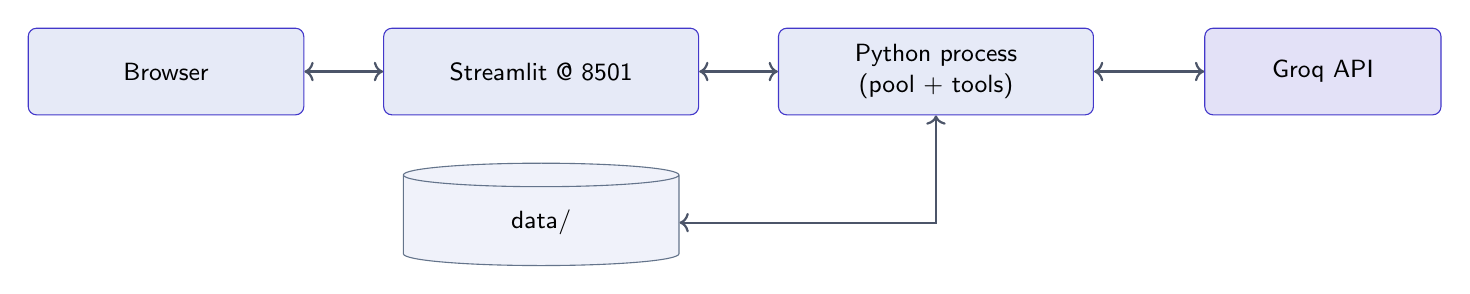
\begin{tikzpicture}[node distance=0.6cm and 1cm, font=\small\sffamily]
  \node[al-node, minimum width=3.5cm] (br) {Browser};
  \node[al-node, right=of br, minimum width=4cm]
                                                (st) {Streamlit @ 8501};
  \node[al-node, right=of st, minimum width=4cm]
                                                (py) {Python process \\ (pool + tools)};
  \node[al-store, below=of st, minimum width=3.5cm]
                                                (fs) {data/};
  \node[al-node, right=1.4cm of py, fill=alAccent!15, minimum width=3cm]
                                                (llm) {Groq API};

  \draw[al-flow, <->] (br) -- (st);
  \draw[al-flow, <->] (st) -- (py);
  \draw[al-flow, <->] (py.south) |- (fs.east);
  \draw[al-flow, <->] (py) -- (llm);
\end{tikzpicture}
\caption{Deployment for the demonstration recording.}
\label{fig:demo-arch}
\end{figure}

\section{Step-by-Step Walkthrough}
\label{sec:walkthrough}

The recommended script is a \textbf{5-minute} demonstration divided
into eight beats.

\subsection*{Beat 1 (0:00--0:30) --- Launch}
Show a terminal executing
\begin{lstlisting}[style=alBash, numbers=none]
streamlit run app/streamlit_app.py
\end{lstlisting}
and highlight the ``Pool ready (in-process): 5/5 services online, 11
unified tools'' log line. Cut to the browser at
\url{http://localhost:8501}.

\begin{figure}[H]
\centering
\fbox{\begin{minipage}{0.9\linewidth}\centering\vspace{6em}
\emph{[SCREENSHOT 1: Streamlit landing page with sidebar showing all
five services in green.]}\vspace{6em}\end{minipage}}
\caption{Landing screen with service health.}
\label{fig:demo-1}
\end{figure}

\subsection*{Beat 2 (0:30--1:00) --- Upload a dataset}
Drag Iris CSV into the sidebar uploader. Show the success toast and
the ``Active dataset'' selector automatically switching to the new
file.

\begin{figure}[H]
\centering
\fbox{\begin{minipage}{0.9\linewidth}\centering\vspace{6em}
\emph{[SCREENSHOT 2: Sidebar showing iris.csv selected as active,
services still green.]}\vspace{6em}\end{minipage}}
\caption{Post-upload sidebar.}
\label{fig:demo-2}
\end{figure}

\subsection*{Beat 3 (1:00--1:45) --- Ask for EDA}
In the chat, type:
\begin{quote}
\emph{``Run a full EDA on my data and summarise what stands out.''}
\end{quote}
Show the tool activity ribbon --- \tool{ingest\_dataset} then
\tool{run\_full\_eda} --- and the assistant's summary paragraphs.
Expand the tool-call cards to reveal the arguments and the JSON
result.

\begin{figure}[H]
\centering
\fbox{\begin{minipage}{0.9\linewidth}\centering\vspace{6em}
\emph{[SCREENSHOT 3: Chat with EDA tool cards expanded and a
correlation heatmap rendered.]}\vspace{6em}\end{minipage}}
\caption{EDA response with expanded tool cards.}
\label{fig:demo-3}
\end{figure}

\subsection*{Beat 4 (1:45--2:45) --- Train a model}
Type:
\begin{quote}
\emph{``Now train a model to predict Species and show me the
leaderboard.''}
\end{quote}
Show the live progress indicator counting up as
\tool{run\_parallel\_bake\_off} completes, then the assistant's
leaderboard summary. Emphasise that the champion is reported
verbatim from the tool result, not fabricated.

\subsection*{Beat 5 (2:45--3:15) --- Explain the model}
Type:
\begin{quote}
\emph{``Explain the champion --- which features matter most?''}
\end{quote}
Depending on the champion, the LLM will call either
\tool{calculate\_shap\_values} or
\tool{generate\_feature\_importance\_plot}. Show the resulting
importance plot inline.

\subsection*{Beat 6 (3:15--3:45) --- Generate a notebook + PDF}
Type:
\begin{quote}
\emph{``Generate a Jupyter notebook that reproduces this pipeline
and a PDF report of the results.''}
\end{quote}
Show \tool{generate\_jupyter\_notebook} and
\tool{compile\_pdf\_report} firing.

\subsection*{Beat 7 (3:45--4:30) --- Browse artefacts}
Switch to the \emph{Artifacts} tab. Show the filter chips, the
image previews for the plots, the parquet dataframe preview for the
\code{xtrain\_sample}, and the download buttons.

\begin{figure}[H]
\centering
\fbox{\begin{minipage}{0.9\linewidth}\centering\vspace{6em}
\emph{[SCREENSHOT 4: Artifacts tab showing at least six artefacts
across the plots, model, notebook, and report categories.]}\vspace{6em}\end{minipage}}
\caption{Artefacts tab after a full run.}
\label{fig:demo-4}
\end{figure}

\subsection*{Beat 8 (4:30--5:00) --- Open the downloads}
Cut to the OS file explorer showing \file{data/artifacts/plots/},
\file{data/artifacts/models/}, \file{data/artifacts/notebooks/},
and \file{data/artifacts/reports/}. Open the generated
\file{.ipynb} in Jupyter to prove it is executable, and the PDF in
a viewer to prove the leaderboard is present.

\section{Expected Terminal Output}
\label{sec:terminal-output}

For reference, the truncated log for a complete run resembles the
following (elided for brevity):

\begin{lstlisting}[style=alBash, numbers=none]
mcp.pool | Pool ready (in-process): 5/5 services online, 11 unified tools
mcp_data | Processing request of type CallToolRequest    # ingest
workspace | Artifact saved: kind=plot id=...             # correlation matrix
workspace | Artifact saved: kind=plot id=...             # distributions
workspace | Artifact saved: kind=plot id=...             # missing values
mcp_data | Processing request of type CallToolRequest    # bake-off
context.py Sending INFO to client: Detected problem type: classification
context.py Sending INFO to client: Training 4 models in parallel
context.py Sending INFO to client: Champion: LightGBM
workspace | Artifact saved: kind=model id=...
workspace | Artifact saved: kind=xtrain_sample id=...
workspace | Artifact saved: kind=plot id=...             # SHAP summary
workspace | Artifact saved: kind=training_notebook id=...
workspace | Artifact saved: kind=pdf_report id=...
\end{lstlisting}

\section{Post-Recording Editing Notes}
\label{sec:post-record}

Recommendations for the video edit:

\begin{itemize}[leftmargin=1.4em]
  \item Overlay the assistant's summary paragraphs at $1.5\times$
        playback while narrating; the raw generation speed varies
        with Groq load.
  \item Highlight the ``\code{artifact\_id}'' fields in the tool
        result to show that every artefact has a stable identifier.
  \item Show the size of \file{data/artifacts/\_index.json} growing
        after each artefact save --- this makes the registry
        tangible.
\end{itemize}

\chapter{Limitations}
\label{ch:limitations}

This chapter states the limitations of \projname{} honestly. Each
item is either an intentional trade-off, a scope decision, or an
open technical issue. Every claim in this chapter is verifiable from
the current repository.

\section{Data Modality Limitations}
\label{sec:lim-data}

\begin{itemize}[leftmargin=1.4em]
  \item \textbf{Tabular only.} The pipeline assumes rectangular
        pandas-friendly data. Text, images, audio, time series,
        and graphs are out of scope.
  \item \textbf{Single-file datasets.} Multi-table joins, relational
        databases, and streaming data are not supported.
  \item \textbf{Memory-bound.} Datasets are loaded whole with
        \code{pandas.read\_csv} or \code{read\_parquet}. Extremely
        wide or extremely long datasets can exhaust RAM before the
        upload cap is reached.
\end{itemize}

\section{Compute Limitations}
\label{sec:lim-compute}

\begin{itemize}[leftmargin=1.4em]
  \item \textbf{CPU only.} The recommended install path does not
        include GPU-enabled builds of XGBoost or LightGBM. Users can
        install them separately, but no CUDA integration is provided
        out of the box.
  \item \textbf{No distributed training.} Bake-off parallelism is
        limited to a single machine and $\le 4$ candidate threads.
  \item \textbf{Single-process Optuna.} The sweep runs with
        \code{n\_jobs=1} at the study level to keep bookkeeping
        simple; multi-process TPE requires shared storage.
\end{itemize}

\section{Model and Algorithm Limitations}
\label{sec:lim-models}

\begin{itemize}[leftmargin=1.4em]
  \item \textbf{Fixed candidate set.} The bake-off compares only
        RandomForest, XGBoost, LightGBM, and a linear baseline
        (LogisticRegression or Ridge). Stacking, blending, deep
        tabular models (e.g.\ TabNet, FT-Transformer), and
        CatBoost are not currently included.
  \item \textbf{No feature engineering search.} Preprocessing is a
        fixed \code{ColumnTransformer}; feature interactions,
        target encoders, and count encoders are not attempted.
  \item \textbf{No calibration or thresholding.} Classification
        outputs are point predictions; probability calibration and
        threshold tuning are not performed.
  \item \textbf{Uni-target regression / classification only.}
        Multi-label, multi-target, and hierarchical tasks are not
        supported.
\end{itemize}

\section{Agent Reliability and Hallucination}
\label{sec:lim-hallucination}

\begin{itemize}[leftmargin=1.4em]
  \item \textbf{Wrong tool selection.} The LLM may occasionally
        choose the wrong tool, e.g.\ calling
        \tool{run\_parallel\_bake\_off} without confirming the
        target column when it should have asked.
  \item \textbf{Argument fabrication.} Free-form arguments such as
        \code{target\_column} are constructed by the LLM. If the
        user's phrasing is ambiguous, the LLM may invent a plausible
        column name; this is why the modeling tool now returns a
        friendly error listing the actual columns
        (Section~\ref{sec:qual-results}).
  \item \textbf{Result misinterpretation.} The LLM may summarise
        tool results incorrectly. This is mitigated by expandable
        tool-call cards in the UI so the user can inspect raw JSON.
  \item \textbf{Iteration ceiling.} Long compound tasks may hit the
        default \code{MAX\_TOOL\_ITERATIONS=8} limit before
        completing; the platform will end with a plain-text apology
        rather than an error.
\end{itemize}

\section{Scalability Limitations}
\label{sec:lim-scale}

\begin{itemize}[leftmargin=1.4em]
  \item \textbf{Single user.} There is no user identity, no
        per-user directory, and no access control. Multi-tenant
        deployment would require reintroducing an auth layer and a
        per-user workspace.
  \item \textbf{Streamlit re-runs.} Streamlit re-runs the whole
        script on every widget event; long tool outputs are
        re-rendered on each re-run.
  \item \textbf{No horizontal scaling.} There is no queue, no
        worker process pool, and no orchestration for concurrent
        chat sessions.
\end{itemize}

\section{Security Limitations}
\label{sec:lim-security}

\begin{itemize}[leftmargin=1.4em]
  \item \textbf{No sandboxing of pandas.} Uploaded files are parsed
        with \code{pandas.read\_csv}, which is safe against arbitrary
        code execution but is exposed to CSV injection into
        downstream tools that consume string values.
  \item \textbf{Attacker-influenced tool results.} Data-derived
        strings are echoed back to the LLM and could contain
        prompt-injection payloads. Mitigation: raw tool results are
        visible in the UI; the platform is not run unattended.
  \item \textbf{Secrets in \file{.env}.} The API key is stored in
        plain text in the working directory. Users should treat
        \file{.env} as sensitive and keep it out of version
        control (the \file{.gitignore} already excludes it).
\end{itemize}

\section{Reproducibility Limitations}
\label{sec:lim-repro}

\begin{itemize}[leftmargin=1.4em]
  \item \textbf{LLM non-determinism.} Even at low temperature,
        Groq's streaming responses vary run to run; the prose is
        not byte-reproducible.
  \item \textbf{Provider drift.} A Groq-side update to
        \code{llama-3.3-70b-versatile} would change behaviour
        without any change in the local repository.
  \item \textbf{No dataset hash.} The platform does not currently
        record a hash of the uploaded dataset. Recomputing artefacts
        after a data change is silent.
\end{itemize}

\section{Dependency Footprint}
\label{sec:lim-deps}

The dependency list (Table~\ref{tab:deps}) is heavy for a research
tool: scikit-learn, XGBoost, LightGBM, SHAP, Optuna, matplotlib, and
ReportLab together account for hundreds of megabytes when installed.
This is intentional --- the platform's value proposition is a
batteries-included pipeline --- but it does mean that installation
is not instantaneous and that Docker images built naively will be
sizable.

\begin{table}[H]
\centering
\caption{Runtime dependencies of \projname{} and their purpose.
Every entry is a direct import in the code.}
\label{tab:deps}
\small
\begin{tabularx}{\linewidth}{@{}lXl@{}}
\toprule
\textbf{Package} & \textbf{Purpose in \projname} & \textbf{Category} \\
\midrule
streamlit & UI                              & UI \\
fastmcp   & MCP servers + in-process transport & Protocol \\
groq      & Chat Completions API client     & LLM \\
numpy, pandas, pyarrow & Data handling      & Data \\
scikit-learn & Preprocessing + ML pipeline  & ML \\
scipy     & Statistical helpers             & ML \\
xgboost, lightgbm & Gradient boosting       & ML \\
shap      & Explainability                  & ML \\
optuna    & Hyperparameter search           & ML \\
pandera   & Schema validation               & Data \\
matplotlib & Plot rendering                 & Viz \\
reportlab & PDF generation                  & Export \\
pydantic, pydantic-settings & Typed config  & Config \\
python-dotenv & \file{.env} loading         & Config \\
\bottomrule
\end{tabularx}
\end{table}

\section{Architectural Limitations}
\label{sec:lim-arch}

\begin{itemize}[leftmargin=1.4em]
  \item \textbf{No message persistence.} Chat history is held in
        Streamlit session state; a page refresh loses it. The
        earlier prototype (removed during migration) persisted
        conversations in a database.
  \item \textbf{No MCP resource endpoints.} The MCP protocol
        supports resources (addressable read-only content) but the
        current servers expose none.
  \item \textbf{No observability stack.} There is no Prometheus
        exporter, no tracing (OpenTelemetry), and no structured
        JSON log output. Only stderr logs are produced.
  \item \textbf{No CI/CD.} There is no automated build, lint, or
        test in the repository.
\end{itemize}

Every limitation above is addressed as future work in
Chapter~\ref{ch:conclusion}, either as a small extension or as a
clearly-labelled research direction.

\chapter{Conclusion and Future Directions}
\label{ch:conclusion}

\section{Summary of Contributions}
\label{sec:sum-contrib}

This report has described the design and implementation of
\projname, a single-machine, local-first, conversational AutoML
platform built on the Model Context Protocol. The concrete
contributions are:

\begin{enumerate}[leftmargin=1.4em]
  \item A modular MCP server layout that decomposes a tabular
        pipeline into five independent services and eleven typed
        tools.
  \item An in-process transport layer that removes HTTP overhead
        while preserving the MCP protocol's discovery and
        invocation semantics.
  \item An orchestrator that reduces the LLM to a
        \emph{scheduler}: it never fabricates numbers, only picks
        tools and arguments and formats their results.
  \item A filesystem artefact registry that gives every generated
        file a UUID, a category, and searchable metadata.
  \item A thin Streamlit UI that is a client of the orchestrator
        and can be replaced without touching the ML code.
\end{enumerate}

\section{Findings}
\label{sec:findings}

The end-to-end smoke of the pipeline confirms three important
findings.

\paragraph{The MCP contract is enough.}
A typed tool schema plus a docstring is sufficient information for
current-generation LLMs to plan multi-step workflows. There is no
need for a bespoke protocol on top of MCP for a research-scale
platform.

\paragraph{Deterministic-first works.}
Restricting the LLM to plan-and-format decisions --- and letting
Python do every calculation --- keeps the platform trustworthy. The
user never has to wonder whether a metric was computed or
hallucinated.

\paragraph{Local-first pays off.}
Removing Supabase, authentication, cloud storage, and the Next.js
frontend cut the surface area by more than half and made the
platform tractable for a single-author project without sacrificing
any pipeline capability.

\section{Future Directions}
\label{sec:future}

The following extensions are natural next steps. Each is labelled
\propd{} if a small effort would deliver it, or \future{} for
larger research or engineering programs.

\subsection{AutoML Depth}
\label{sec:future-automl}

\begin{itemize}[leftmargin=1.4em]
  \item \propd{} Add CatBoost \citep{prokhorenkova2018catboost} as a
        fifth bake-off candidate.
  \item \propd{} Add stacking (\code{StackingClassifier} /
        \code{StackingRegressor} \citep{sklearn2011}) as a
        post-bake-off step.
  \item \future{} Integrate deep tabular models (TabNet
        \citep{arik2021tabnet}, FT-Transformer
        \citep{gorishniy2021revisiting}) as optional candidates
        behind a flag.
  \item \future{} Add multi-fidelity HPO (Hyperband
        \citep{li2017hyperband}, BOHB \citep{falkner2018bohb}).
  \item \future{} Feature engineering search
        (Featuretools-style \citep{kanter2015dsm}, LLM-driven CAAFE
        \citep{hollmann2024caafe}).
\end{itemize}

\subsection{Agent Sophistication}
\label{sec:future-agent}

\begin{itemize}[leftmargin=1.4em]
  \item \propd{} Add ReAct-style scratchpad
        \citep{yao2023react} to the system prompt for better
        multi-step reasoning.
  \item \propd{} Add self-consistency
        \citep{wang2023self-consistency} on tool argument
        generation.
  \item \future{} Multi-agent workflows
        \citep{wu2023autogen, hong2024metagpt}: a Planner that
        proposes a DAG of tool calls and a Critic that reviews
        results before final response.
  \item \future{} Retrieval-augmented tool selection over a larger
        catalog \citep{patil2023gorilla, qin2024toolllm}.
\end{itemize}

\subsection{Reproducibility and MLOps}
\label{sec:future-mlops}

\begin{itemize}[leftmargin=1.4em]
  \item \propd{} Record a SHA-256 hash of every uploaded dataset in
        \code{DatasetRecord} and expose it as an artefact metadata
        field.
  \item \propd{} Store leaderboards in a small SQLite database so
        that historical bake-offs can be queried.
  \item \future{} Integrate with MLflow \citep{mlflow} or Weights
        \& Biases \citep{wandb} for experiment tracking and model
        registry semantics.
  \item \future{} Emit OpenTelemetry \citep{opentelemetry} traces
        for every tool call to enable proper observability.
\end{itemize}

\subsection{Deployment and Scaling}
\label{sec:future-deploy}

\begin{itemize}[leftmargin=1.4em]
  \item \propd{} Provide a minimal \file{Dockerfile} that installs
        \file{requirements.txt} and exposes the Streamlit port.
  \item \future{} Split each MCP server into its own process
        (or container) and re-transport them over Streamable HTTP
        \citep{mcpSpec2024} so they can scale independently.
  \item \future{} Add a job queue (Redis / RQ or Celery
        \citep{celery}) so long-running bake-offs do not block the
        UI thread.
  \item \future{} Cloud deployment templates for AWS ECS, Google
        Cloud Run, or Kubernetes.
\end{itemize}

\subsection{Human-in-the-Loop and Guard-rails}
\label{sec:future-hitl}

\begin{itemize}[leftmargin=1.4em]
  \item \propd{} Add a ``dry-run'' mode in which the LLM emits a
        plan of tool calls that the user must approve before
        execution.
  \item \propd{} Add a policy layer that inspects tool arguments
        (e.g.\ reject \code{target\_column} values that do not
        exist).
  \item \future{} Prompt-injection defence: separate tool results
        into a distinct message channel and re-anchor the system
        prompt on every turn.
\end{itemize}

\subsection{Broader Data Modalities}
\label{sec:future-modality}

\begin{itemize}[leftmargin=1.4em]
  \item \future{} Time-series support (statsforecast
        \citep{statsforecast}, sktime \citep{sktime}).
  \item \future{} Text classification with sentence-transformers
        \citep{reimers2019sbert}.
  \item \future{} Image classification via torchvision-style
        pipelines.
  \item \future{} Multimodal LLM-driven captioning of generated
        plots for accessibility.
\end{itemize}

\subsection{Ecosystem Integration}
\label{sec:future-ecosystem}

\begin{itemize}[leftmargin=1.4em]
  \item \propd{} Expose the MCP servers over stdio as well as
        in-process so that Claude Desktop and other MCP hosts can
        use them.
  \item \propd{} Expose MCP resources for the artefact catalog so
        that any MCP client can \code{ReadResource} the leaderboard
        or the champion metadata.
  \item \future{} Publish the MCP servers as a stand-alone package
        that other AutoML front-ends can consume.
\end{itemize}

\subsection{Benchmarking}
\label{sec:future-bench}

\begin{itemize}[leftmargin=1.4em]
  \item \propd{} Automated CI job that runs the protocol of
        Chapter~\ref{ch:experiments} on all six datasets and posts
        the resulting Markdown table as a comment on every PR.
  \item \future{} Compare \projname{} against AutoGluon
        \citep{erickson2020autogluon}, Auto-sklearn
        \citep{feurer2015autosklearn}, and TPOT
        \citep{olson2016tpot} on OpenML CC-18 benchmarks
        \citep{bischl2021openml}.
\end{itemize}

\section{Closing Remarks}
\label{sec:closing}

Conversational, agentic interfaces to data science are neither a
substitute for statistical intuition nor a solution to the
underlying difficulty of applied ML. What they can do, when
carefully designed, is lower the activation energy for someone who
has intuition but has not yet internalised the API surface --- and
give that person a clean, inspectable, downloadable record of
everything the platform did. \projname{} is a small step in this
direction, built to be extended.


% ---- Appendices -------------------------------------------------
\appendix
\chapter{Project Structure}
\label{app:structure}

The repository shipped alongside this report has the following
layout. Every path is relative to the repository root
\file{automl-mcp-platform/}. Sizes are in lines of Python (LoC).

\begin{lstlisting}[style=alBash, caption={Repository tree.},
                    label={lst:tree-app}]
automl-mcp-platform/
|-- app/
|   |-- __init__.py                  (0)
|   |-- streamlit_app.py             (~345 LoC)
|   `-- components/                  (reserved for render helpers)
|-- core/
|   |-- __init__.py                  (0)
|   |-- config.py                    (~52 LoC)
|   |-- logger.py                    (~19 LoC)
|   `-- workspace.py                 (~252 LoC)
|-- mcp_servers/
|   |-- __init__.py                  (0)
|   |-- data.py                      (~180 LoC)
|   |-- eda.py                       (~336 LoC)
|   |-- modeling.py                  (~388 LoC)
|   |-- explain.py                   (~197 LoC)
|   `-- export.py                    (~284 LoC)
|-- orchestrator/
|   |-- __init__.py                  (~5 LoC)
|   |-- pool.py                      (~288 LoC)
|   `-- loop.py                      (~295 LoC)
|-- data/
|   |-- uploads/    (raw CSV / TSV / Parquet)
|   |-- artifacts/  (plots, models, notebooks, reports)
|   `-- tmp/        (per-service scratch)
|-- .env.example
|-- .gitignore
|-- LICENSE                          (Apache-2.0)
|-- README.md
`-- requirements.txt
\end{lstlisting}

\section*{Total Codebase Size}

\begin{table}[H]
\centering
\caption{Lines of Python by package.}
\label{tab:loc}
\begin{tabular}{@{}lr@{}}
\toprule
\textbf{Package} & \textbf{LoC (approx.)} \\
\midrule
\file{core/}         & 323 \\
\file{mcp\_servers/} & 1\,385 \\
\file{orchestrator/} & 588 \\
\file{app/}          & 345 \\
\midrule
\textbf{Total}       & \textbf{2\,641} \\
\bottomrule
\end{tabular}
\end{table}

\chapter{Configuration Reference}
\label{app:config}

Every configuration setting is loaded from the \file{.env} file in
the repository root through \code{pydantic-settings}
\citep{pydantic}. The complete list is reproduced below and matches
\file{core/config.py}.

\begin{table}[H]
\centering
\caption{Configuration variables (all read from \file{.env}).}
\label{tab:config}
\small
\begin{tabularx}{\linewidth}{@{}lXl@{}}
\toprule
\textbf{Variable} & \textbf{Purpose} & \textbf{Default} \\
\midrule
\code{GROQ\_API\_KEY} & Groq API key. Required for chat/orchestration; if empty, the UI shows an error banner and disables the chat input. & \emph{(empty)} \\
\code{GROQ\_MODEL} & Groq model identifier used by the tool-call loop. & \code{llama-3.3-70b-versatile} \\
\code{MAX\_TOOL\_ITERATIONS} & Maximum number of outer loop iterations per user turn. & \code{8} \\
\code{MAX\_UPLOAD\_MB} & Upload size cap enforced client-side in the Streamlit sidebar. & \code{200} \\
\code{DATA\_DIR} & Root directory for \file{uploads/}, \file{artifacts/}, and \file{tmp/}. Absolute or relative to the repository. & \code{./data} \\
\bottomrule
\end{tabularx}
\end{table}

\section*{Sample \file{.env.example}}

\begin{lstlisting}[style=alBash, caption={Contents of \file{.env.example}.}, label={lst:env}]
# Groq LLM (required for chat/orchestration)
GROQ_API_KEY=gsk_your_key_here
GROQ_MODEL=llama-3.3-70b-versatile

# Orchestrator behavior
MAX_TOOL_ITERATIONS=8
MAX_UPLOAD_MB=200

# Where uploaded datasets, generated artifacts, and tmp files live.
# Leave commented to use ./data at the repo root.
# DATA_DIR=./data
\end{lstlisting}

\section*{Derived Paths}

\code{Settings} exposes the following properties, each of which
creates the underlying directory on first access:

\begin{itemize}[leftmargin=1.4em]
  \item \code{settings.data\_path} $\to$ \file{./data}
  \item \code{settings.uploads\_path} $\to$ \file{./data/uploads}
  \item \code{settings.artifacts\_path} $\to$ \file{./data/artifacts}
  \item \code{settings.tmp\_path} $\to$ \file{./data/tmp}
\end{itemize}

\chapter{Public API and MCP Tool Catalog}
\label{app:api}

\section{Python API}
\label{sec:api}

The orchestrator package exposes three symbols that make up the
platform's Python API:

\begin{lstlisting}[caption={\file{orchestrator/\_\_init\_\_.py}.},
label={lst:api}]
from orchestrator.loop import stream_chat
from orchestrator.pool import MCPClientPool, register_default_servers

__all__ = ["stream_chat", "MCPClientPool", "register_default_servers"]
\end{lstlisting}

A minimal programmatic session:

\begin{lstlisting}[caption={Minimal script using the Python API.},
label={lst:api-usage}]
import asyncio
from orchestrator import MCPClientPool, register_default_servers, stream_chat

async def main():
    pool = MCPClientPool()
    register_default_servers(pool)
    await pool.start()

    async for evt in stream_chat(
        query="Run EDA on iris.csv",
        active_file="iris.csv",
        history=[],
        pool=pool,
    ):
        print(evt)

    await pool.shutdown()

asyncio.run(main())
\end{lstlisting}

Direct tool invocation is also possible without the LLM in the
loop:

\begin{lstlisting}[caption={Direct MCP tool call (bypasses the LLM).},
label={lst:direct}]
result = await pool.call_tool(
    "ingest_dataset", {"file_path": "iris.csv"})
print(result.structured_content)
\end{lstlisting}

\section{MCP Tool Catalog}
\label{sec:tool-catalog}

Table~\ref{tab:tool-catalog} lists every tool with its owning
service, required arguments, and return summary. The full JSON
schemas are auto-generated by FastMCP from the Python type hints
and docstrings and are visible inside the running app on the
\emph{Tools} tab.

\begin{table}[H]
\centering
\caption{Complete MCP tool catalog.}
\label{tab:tool-catalog}
\small
\begin{tabularx}{\linewidth}{@{}llXX@{}}
\toprule
\textbf{Service} & \textbf{Tool} & \textbf{Required args} & \textbf{Returns (summary)} \\
\midrule
mcp-data & \tool{list\_uploaded\_files} & --- & \code{count}, \code{files[]} \\
mcp-data & \tool{ingest\_dataset} & \code{file\_path} & shape, dtypes, head, missing, duplicates \\
mcp-data & \tool{validate\_schema\_with\_pandera} & \code{file\_path} & \code{valid}, inferred rules, failure cases \\
mcp-eda & \tool{run\_full\_eda} & \code{file\_path} & stats, missing summary, 3 plot artefacts \\
mcp-eda & \tool{render\_correlation\_matrix} & \code{file\_path} & method, columns, plot artefact, strong pairs \\
mcp-modeling & \tool{run\_parallel\_bake\_off} & \code{file\_path}, \code{target\_column} & leaderboard, champion, model \& xtrain artefact IDs \\
mcp-modeling & \tool{trigger\_hyperparameter\_sweep} & \code{file\_path}, \code{target\_column}, \code{model\_family} & best value, best params, trial count \\
mcp-explain & \tool{calculate\_shap\_values} & \code{model\_id}, \code{x\_train\_sample\_id} & plot artefact, global importance, explainer kind \\
mcp-explain & \tool{generate\_feature\_importance\_plot} & \code{model\_id} & plot artefact, top-$k$ features \\
mcp-export & \tool{generate\_jupyter\_notebook} & \code{file\_path}, \code{target\_column}, \code{problem\_type} & notebook artefact, cell count \\
mcp-export & \tool{compile\_pdf\_report} & \code{project\_title}, \code{file\_path}, \code{target\_column}, \code{leaderboard}, \code{champion\_model} & PDF artefact \\
\bottomrule
\end{tabularx}
\end{table}

\section{MCP Prompts}
\label{sec:prompts}

The platform ships with one prompt template:

\begin{itemize}[leftmargin=1.4em]
  \item \tool{eda\_deep\_dive(file\_path, target\_column="")} ---
        instructs the LLM to call \tool{run\_full\_eda},
        \tool{render\_correlation\_matrix}, and summarise strong
        correlations, skewed features, and next-step recommendations.
\end{itemize}

\chapter{Reproducibility Notes}
\label{app:repro}

This appendix collects the information required to reproduce any run
of the platform.

\section{Environment Snapshot}
\label{sec:env-snapshot}

The recommended way to snapshot the environment is:

\begin{lstlisting}[style=alBash, numbers=none]
python -V > env.txt
pip freeze >> env.txt
\end{lstlisting}

Store \file{env.txt} alongside the artefacts of the run.

\section{Full Install Sequence}
\label{sec:install}

\begin{lstlisting}[style=alBash, numbers=none]
git clone <repo-url>
cd automl-mcp-platform
python -m venv .venv

# Windows PowerShell
.venv\Scripts\Activate.ps1
# macOS / Linux
source .venv/bin/activate

pip install -r requirements.txt
cp .env.example .env
# Edit .env to set GROQ_API_KEY

streamlit run app/streamlit_app.py
\end{lstlisting}

\section{Ports and Endpoints}
\label{sec:ports}

\begin{itemize}[leftmargin=1.4em]
  \item Streamlit default: \code{http://localhost:8501}. Override with
        \code{streamlit run app/streamlit\_app.py --server.port 8600}.
  \item Groq: \code{https://api.groq.com} outbound only.
  \item No inbound ports opened by the MCP layer (in-process
        transport).
\end{itemize}

\section{Data Cleanup}
\label{sec:cleanup}

To reset the platform to a clean state:

\begin{lstlisting}[style=alBash, numbers=none]
rm -rf data/uploads/* data/artifacts/* data/tmp/*
touch data/uploads/.gitkeep data/artifacts/.gitkeep data/tmp/.gitkeep
\end{lstlisting}

The \file{.gitkeep} files preserve the directories in Git.

\section{Random Seed Discipline}
\label{sec:seed}

Every tool that involves randomness accepts a
\code{random\_state} argument with default \code{42}. To make a
particular run deterministic under this convention:

\begin{itemize}[leftmargin=1.4em]
  \item Pass the same \code{random\_state} to
        \tool{run\_parallel\_bake\_off} and
        \tool{trigger\_hyperparameter\_sweep}.
  \item Note that \code{n\_jobs=-1} inside individual estimators
        introduces some threading-related non-determinism; for
        strict reproducibility, use \code{n\_jobs=1}.
  \item The LLM output is inherently non-deterministic and is not
        seeded.
\end{itemize}

\chapter{Additional Results (Templates)}
\label{app:extra}

This appendix hosts the numerical results that are produced when the
protocol of Chapter~\ref{ch:experiments} is executed. All tables are
intentionally left with placeholder cells so that the report remains
truthful; users of the platform can fill them in after running the
protocol.

\section{Per-Dataset Leaderboards}
\label{sec:per-dataset}

\begin{table}[H]
\centering
\caption{Leaderboard template. Repeat one such table per dataset.}
\label{tab:per-lb}
\small
\begin{tabularx}{\linewidth}{@{}rlXcccc@{}}
\toprule
\textbf{Rank} & \textbf{Model} & \textbf{Primary metric} & \textbf{CV mean} & \textbf{CV std} & \textbf{Test} & \textbf{Time (s)} \\
\midrule
1 & --- & --- & --- & --- & --- & --- \\
2 & --- & --- & --- & --- & --- & --- \\
3 & --- & --- & --- & --- & --- & --- \\
4 & --- & --- & --- & --- & --- & --- \\
\bottomrule
\end{tabularx}
\end{table}

\section{HPO Sweep Records}
\label{sec:hpo-records}

\begin{table}[H]
\centering
\caption{Optuna sweep template.}
\label{tab:hpo}
\begin{tabular}{@{}lccc@{}}
\toprule
\textbf{Family} & \textbf{Trials} & \textbf{Best CV} & \textbf{Wall time (s)} \\
\midrule
RandomForest & --- & --- & --- \\
XGBoost      & --- & --- & --- \\
LightGBM     & --- & --- & --- \\
\bottomrule
\end{tabular}
\end{table}

\section{Artefact Counts}
\label{sec:artefact-counts}

\begin{table}[H]
\centering
\caption{Artefact counts per dataset after a complete run.}
\label{tab:artefacts}
\begin{tabular}{@{}lccccc@{}}
\toprule
\textbf{Dataset} & \textbf{plots} & \textbf{models} & \textbf{xtrain} & \textbf{notebooks} & \textbf{reports} \\
\midrule
Iris & --- & --- & --- & --- & --- \\
Wine & --- & --- & --- & --- & --- \\
Breast Cancer & --- & --- & --- & --- & --- \\
Adult & --- & --- & --- & --- & --- \\
California Housing & --- & --- & --- & --- & --- \\
\bottomrule
\end{tabular}
\end{table}

\section{LLM Behavioural Scores}
\label{sec:llm-scores}

\begin{table}[H]
\centering
\caption{LLM rubric (see Table~\ref{tab:llm-eval-rubric}) applied
across a prompt suite of size $N$.}
\label{tab:llm-scores}
\begin{tabularx}{\linewidth}{@{}Xccccc@{}}
\toprule
\textbf{Dimension} & \textbf{Iris} & \textbf{Wine} & \textbf{Breast} & \textbf{Adult} & \textbf{Cal.\ Housing} \\
\midrule
Tool selection      & --- & --- & --- & --- & --- \\
Argument fidelity   & --- & --- & --- & --- & --- \\
Composition         & --- & --- & --- & --- & --- \\
Result grounding    & --- & --- & --- & --- & --- \\
Failure handling    & --- & --- & --- & --- & --- \\
Formatting quality  & --- & --- & --- & --- & --- \\
\bottomrule
\end{tabularx}
\end{table}


% ---- Bibliography ----------------------------------------------
\cleardoublepage
\phantomsection
\addcontentsline{toc}{chapter}{Bibliography}
\bibliography{bibliography/references}

\end{document}
